\chapter{Evaluation}
\label{chapter:evaluation}

Before analyzing the work done in this thesis, the depth acquisition pipeline, consisting of the SFM and LSD algorithms, is discussed.

\section{SFM Insufficiencies}\label{subsec:sfm_insufficiencies}
SFM is part of the LORNA pipeline and promises to be a valid option for the tackled endeavor. Before this work however, it was never tested extensively, especially at high altitudes (100 m).

\begin{figure}[h]
\centering
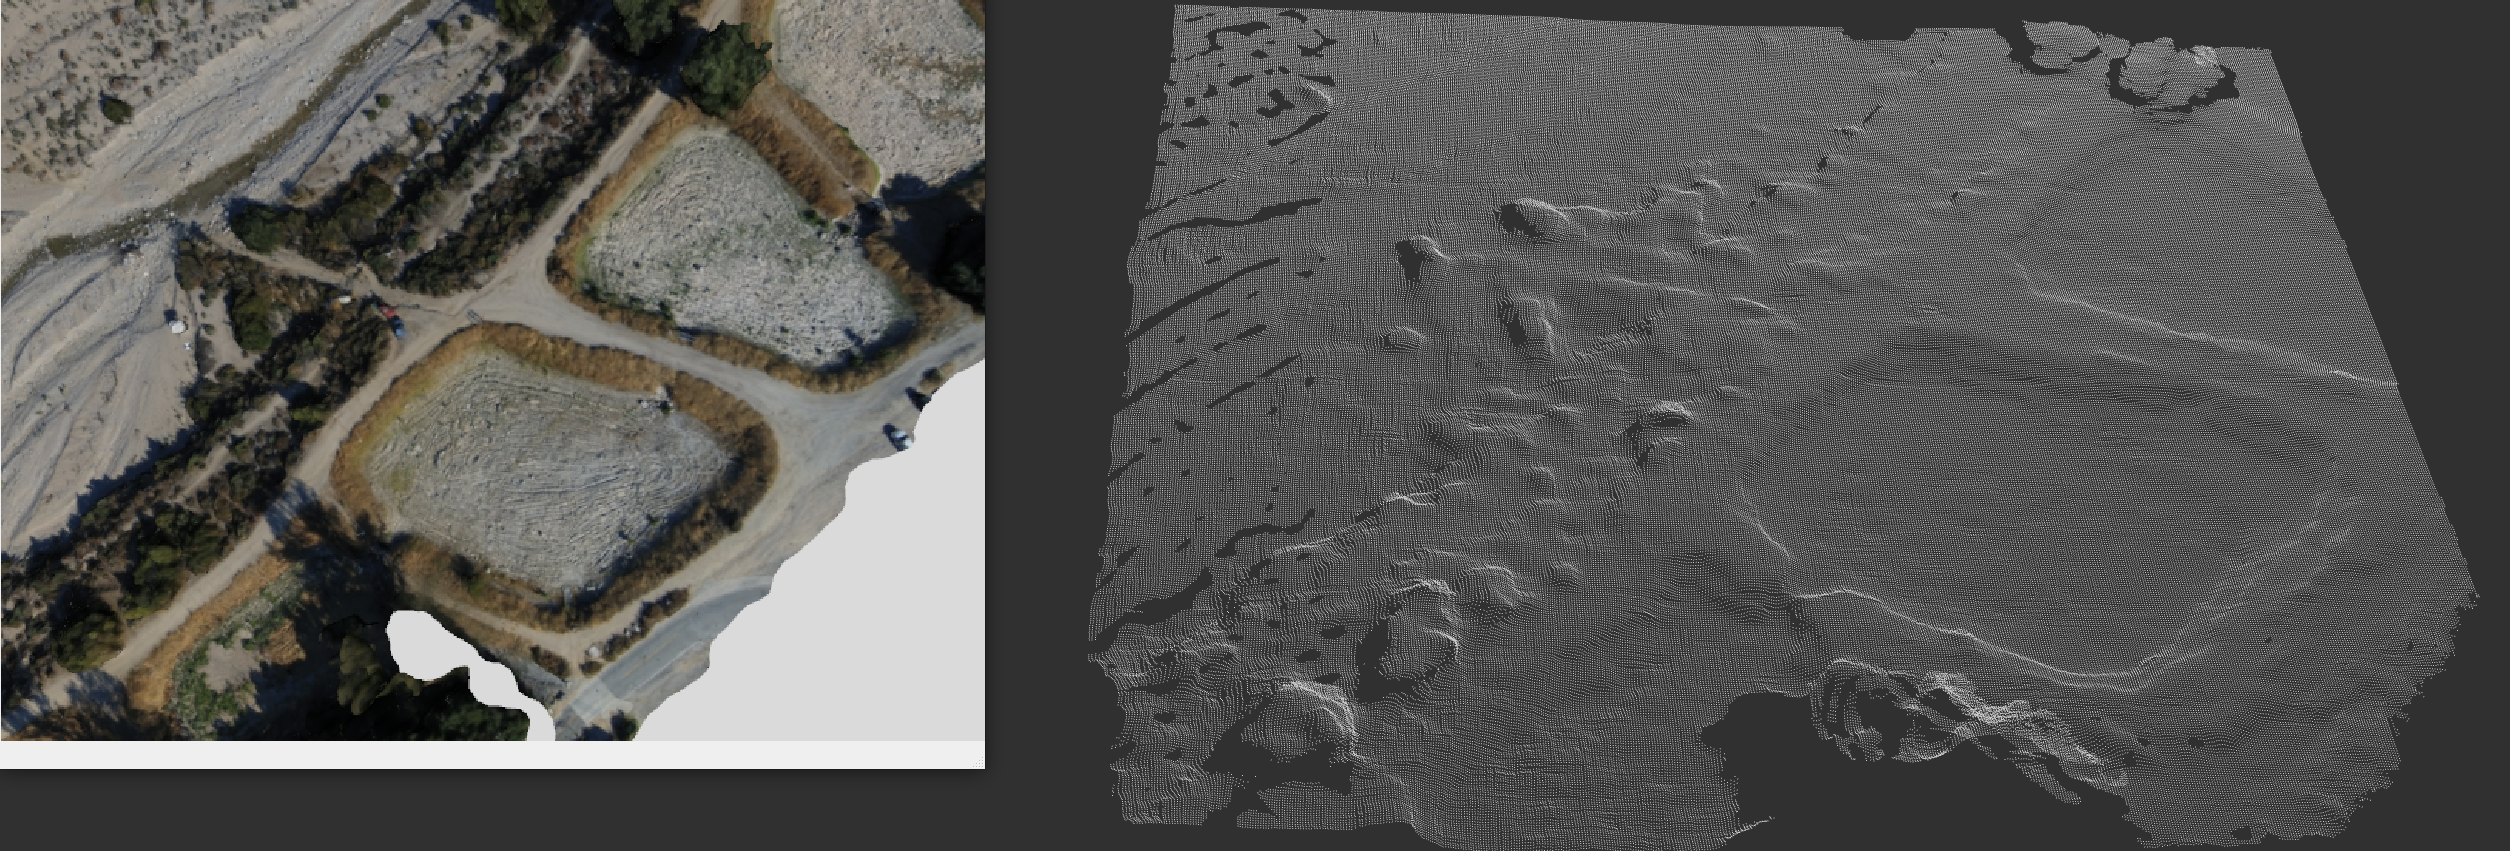
\includegraphics[scale=0.14]{images/evaluation/SFM_issues/SFM_quality.png}
\caption{SFM point cloud when initialized correctly - left: SFM's input image, right: SFM's point cloud output visualized in rviz}
\label{fig:sfm_quality}
\end{figure}

Looking at \cref{fig:sfm_quality}, it is fair to say that SFM is capable of creating accurate point clouds at high altitudes. Though performing well when initialized successfully, SFM often had issues during startup and showed frequent insufficiencies during rotations or, in general, high-altitude flights.

Unfortunately, a lack of time prevented me from investigating these issues in detail. Nevertheless, the shortcomings of the current standing are laid out to the best of my knowledge in the following to hopefully be resolved in future work.

SFM's main issues occurred in the following three scenarios:

\begin{itemize}
    \item During startup

    Frequently, when starting SFM's keyframe recording, it would not start or output corrupted data, especially when there was slight rotation in the drone's movement. When making sure that SFM is initialized during perfect lateral motion, the initialization succeeded most often. This leads to a strong suspicion that SFM handles rotations poorly during initialization.
    \item When changing direction

    Most often, the drone is in vertical or straight, lateral movement. However, it has to turn between waypoints or landing site attempts. Currently, SFM isn't able to handle these cases well. As for the initialization, it either stops or outputs faulty data. A demonstration of SFM outputting point clouds and stopping upon changing direction is shown in \cref{fig:sfm_stop}. An example of corrupted input data is shown in \cref{fig:sfm_fault} and \cref{fig:SFM_issue_1}. Note how in \cref{fig:SFM_issue_1} SFM started producing invalid data after a map move. Furthermore, \cref{fig:sfm_pc_fault1} and \cref{fig:sfm_pc_fault2} depict two instances of faulty point clouds created by SFM.
    \item During high-altitude flights
    
    As mentioned in \cref{subsubsec:SFM_stereo}, SFM often creates point clouds using the same keyframe until it can't establish sufficient image overlap with incoming images anymore and the oldest keyframe is switched. At high altitudes, this leads to frequent, large map movements in LSD as outlined in \cref{subsubsec:setup:aggregation}. As a result of this, LSD's elevation map has a harder time converging, and fewer landing sites are detected. This phenomenon is shown in \cref{fig:SFM_movement1}, \cref{sec:eval_LSD} and \cref{sec:layers}.
\end{itemize}

\begin{figure}[h]
    \centering
    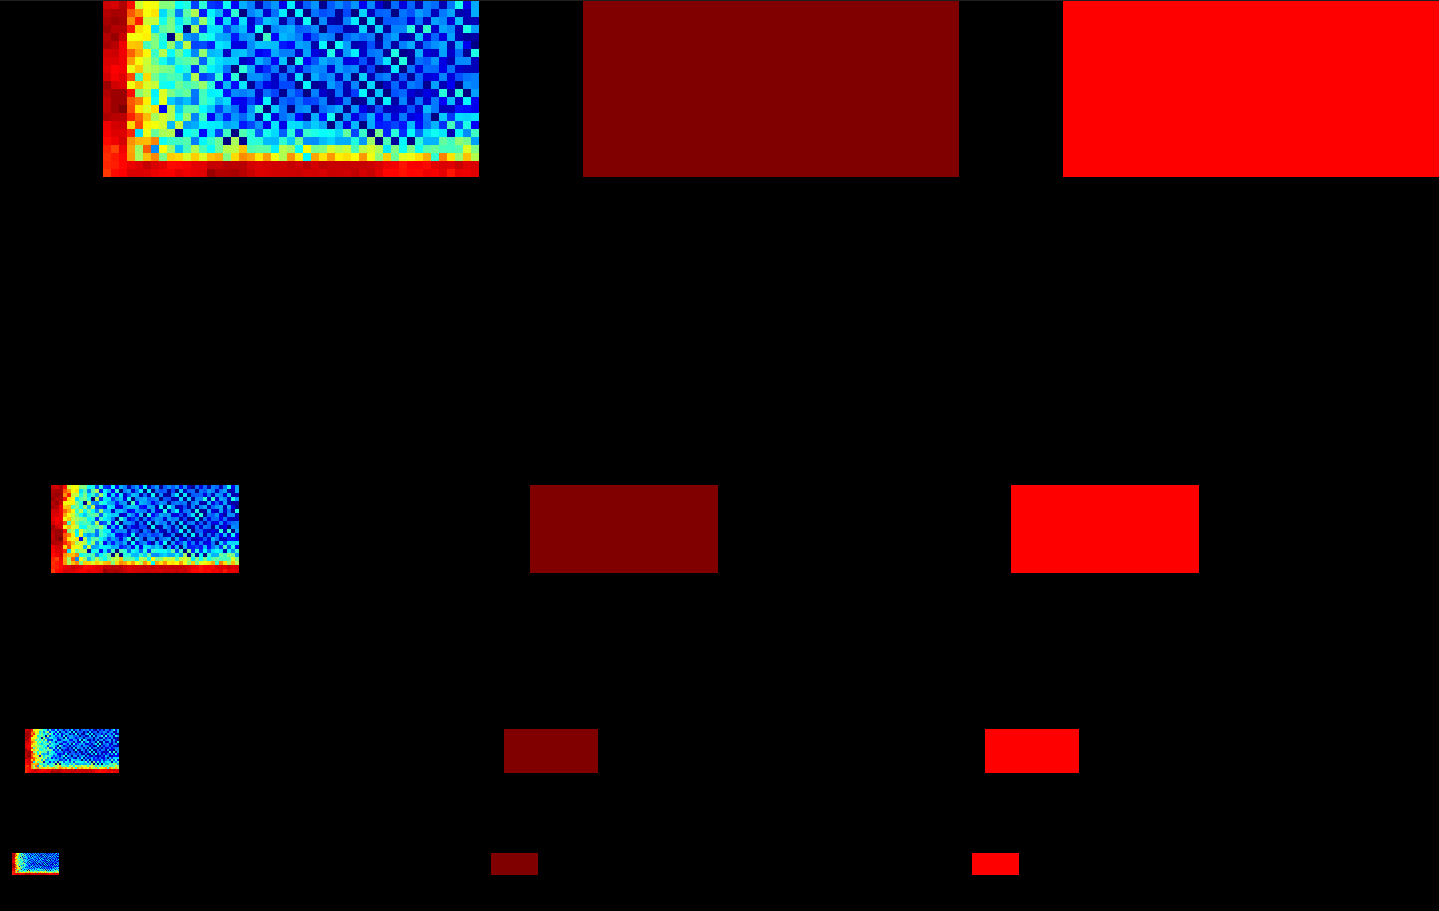
\includegraphics[scale=0.25]{images/evaluation/SFM_issues/sfm_stopped.png}
    \caption{LSD debug image after changing direction: SFM stopped to generate stereo points so that the LSD map is moved without new information coming in.}
    \label{fig:sfm_stop}
\end{figure}

\begin{figure}[h]
    \centering
    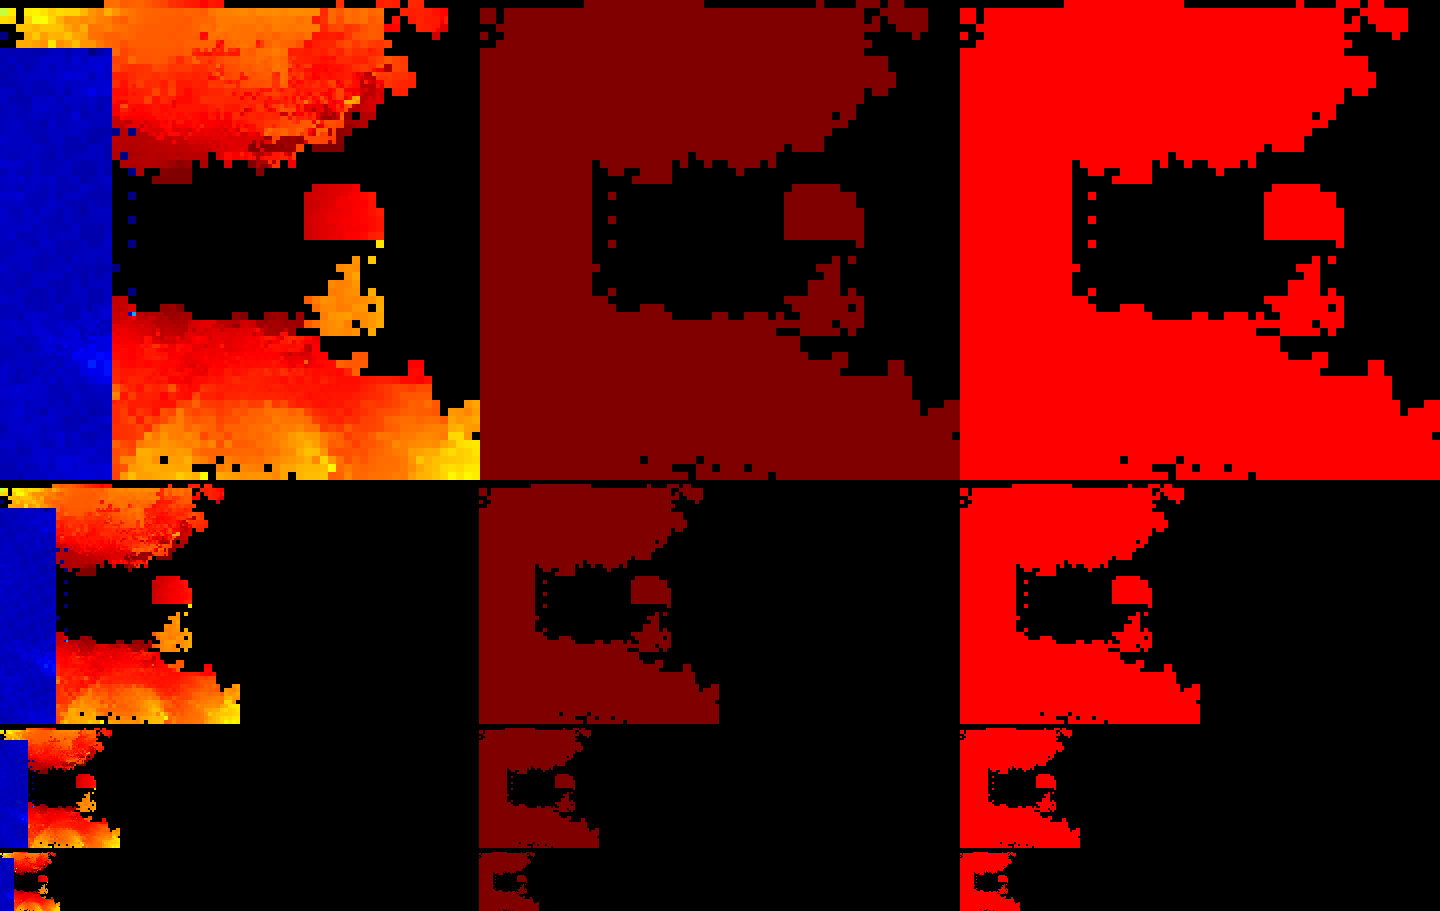
\includegraphics[scale=0.25]{images/evaluation/SFM_issues/issue1.png}
    \caption{One example of the LSD output when supplied with suboptimally performing SFM}
    \label{fig:SFM_issue_1}
\end{figure} 

\begin{figure}[h]
    \centering
    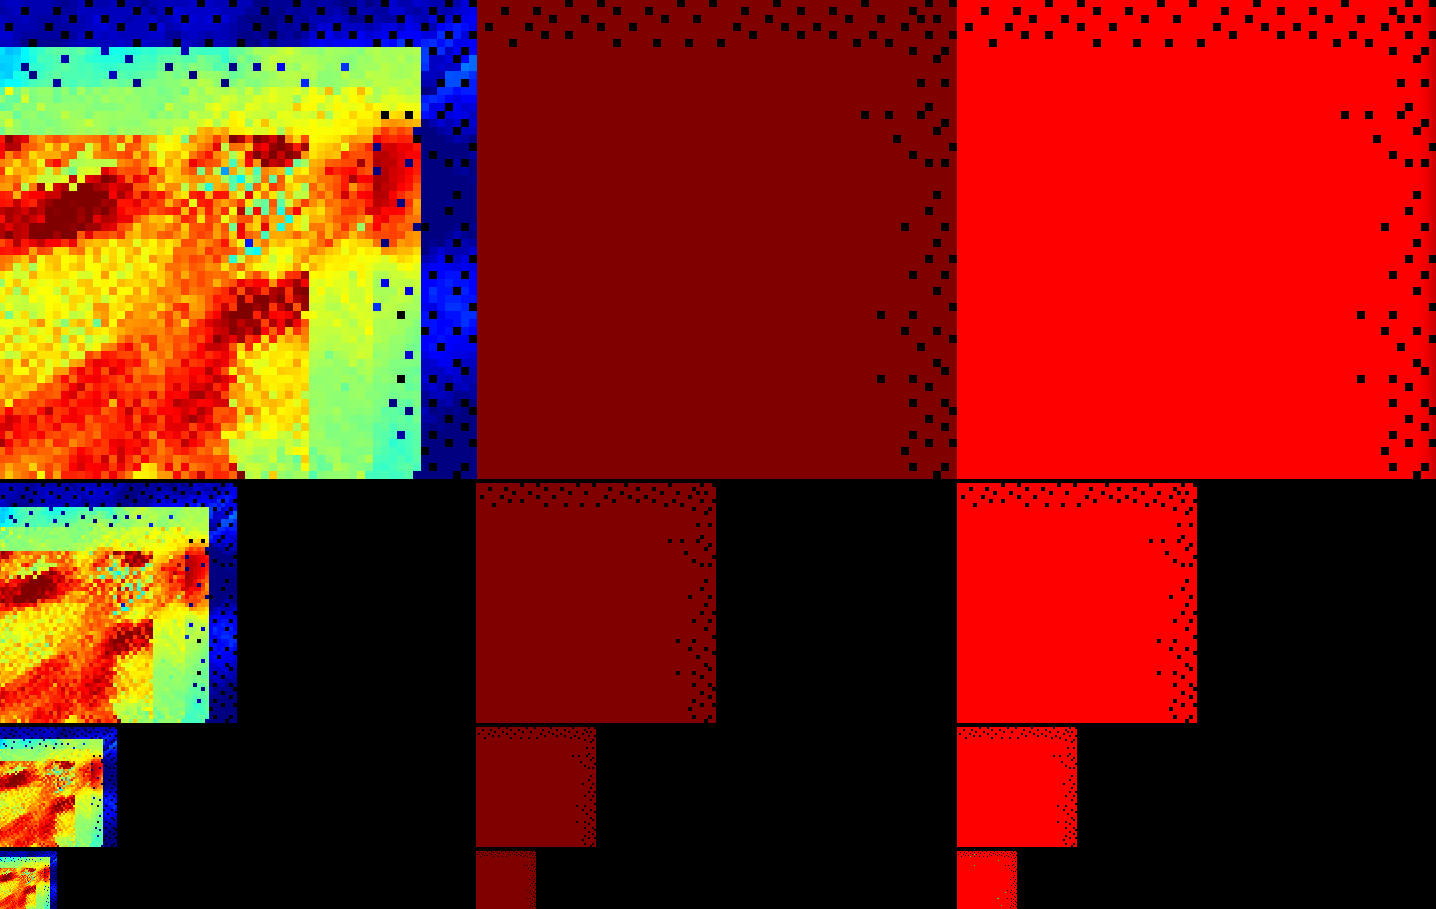
\includegraphics[scale=0.25]{images/evaluation/SFM_issues/issue2.png}
    \caption{Intermediate LSD state after map movement}
    \label{fig:SFM_movement1}
\end{figure}

\begin{figure}[h]
    \centering
    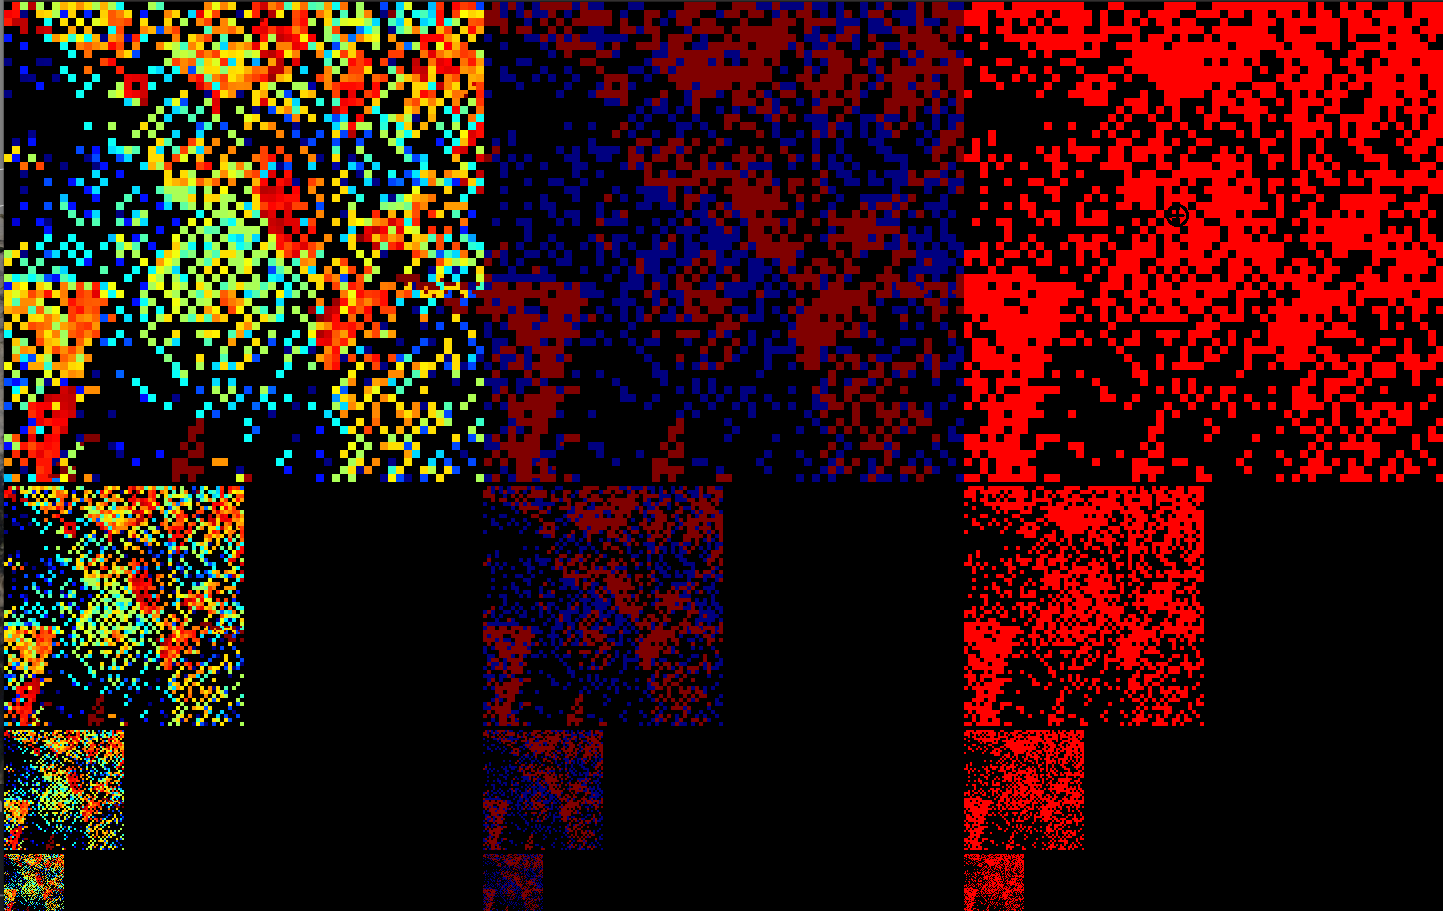
\includegraphics[scale=0.24]{images/evaluation/SFM_issues/sfm_fail.png}
    \caption{Faulty SFM data points generated during flight}
    \label{fig:sfm_fault}
\end{figure}

\begin{figure}[h]
    \centering
    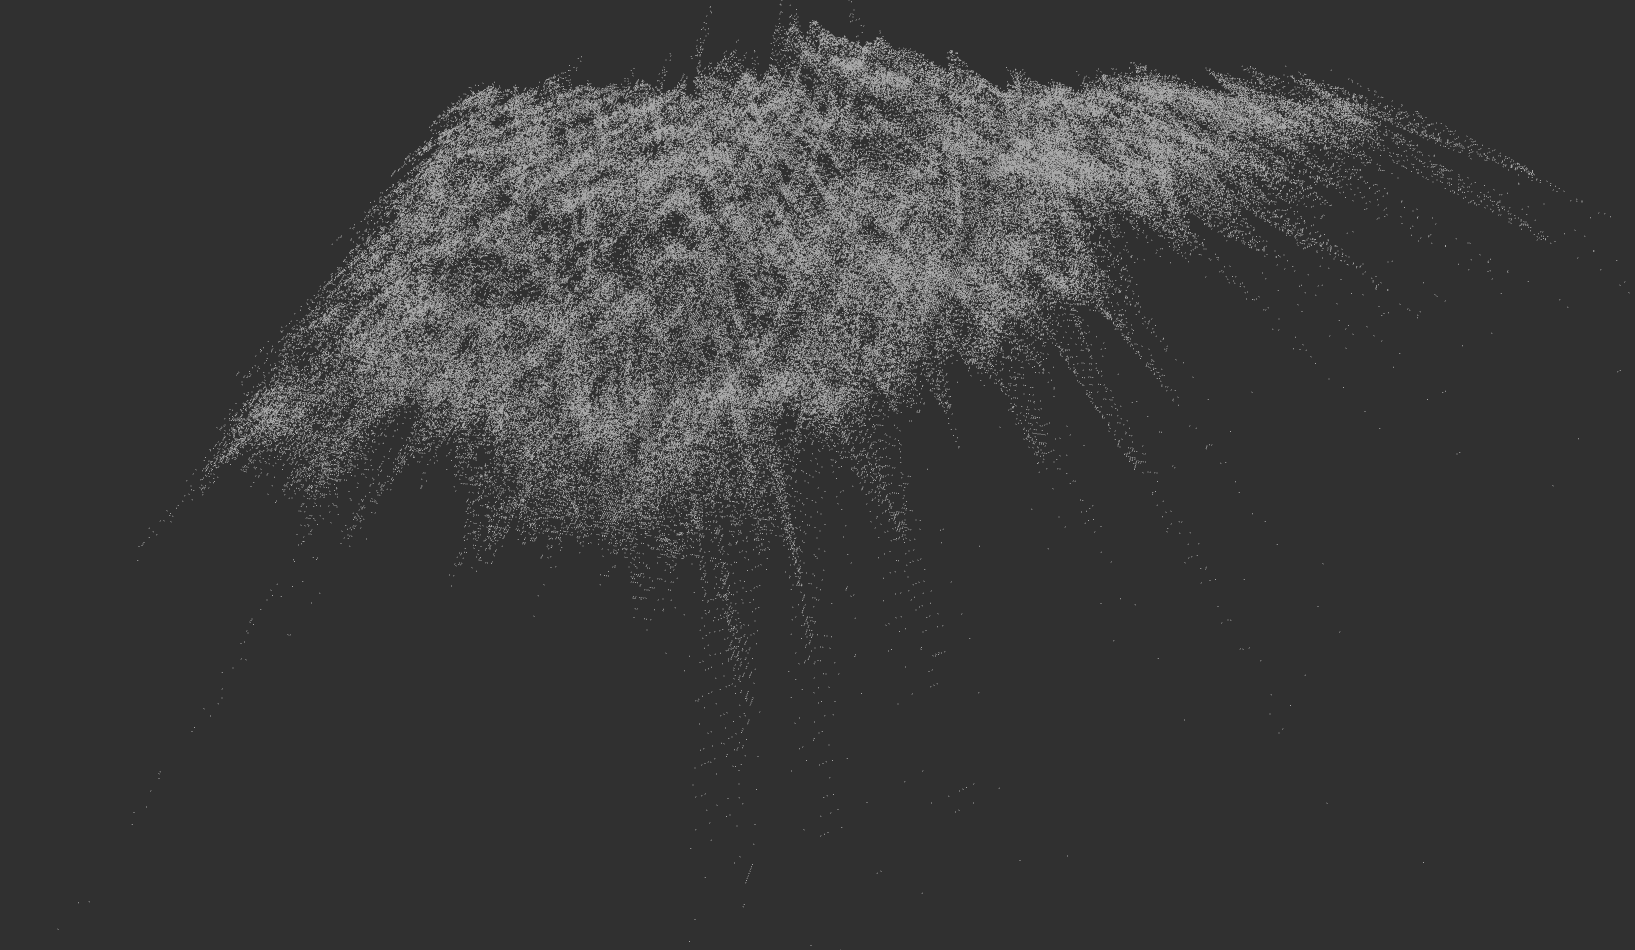
\includegraphics[scale=0.20]{images/evaluation/SFM_issues/sfm_pc_fail1.png}
    \caption{Visualization of faulty SFM point cloud}
    \label{fig:sfm_pc_fault1}
\end{figure}

\begin{figure}[h]
    \centering
    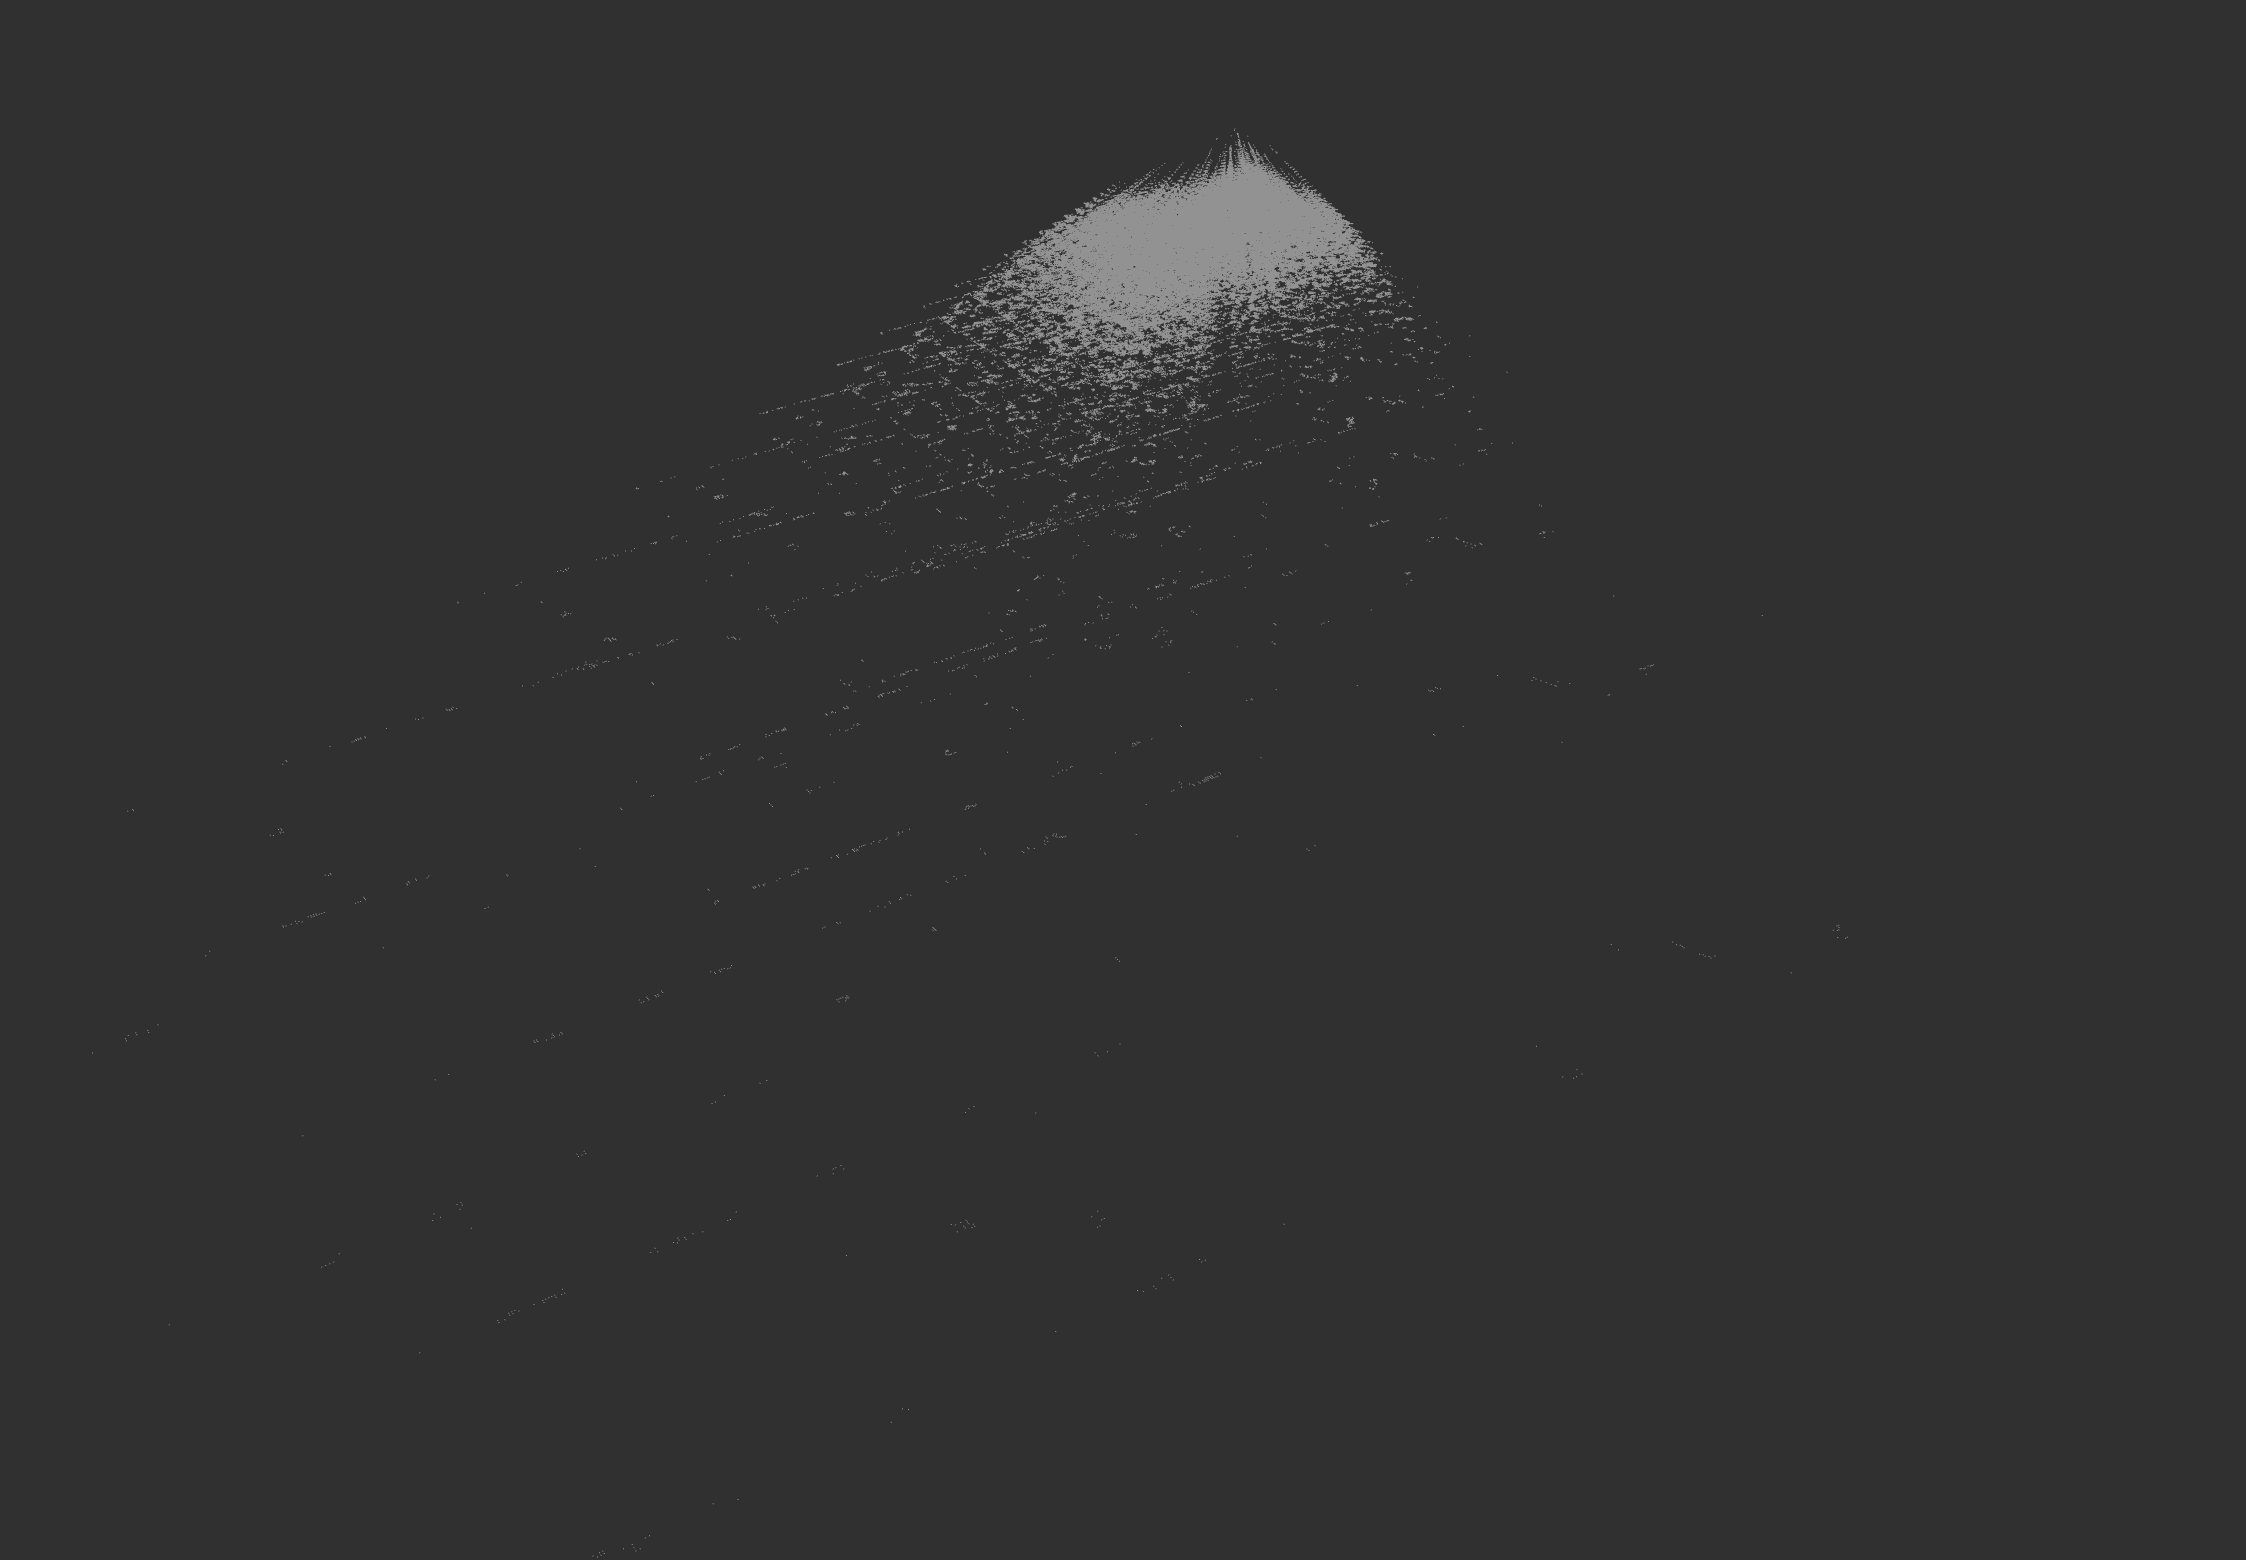
\includegraphics[scale=0.15]{images/evaluation/SFM_issues/sfm_pc_fail2.png}
    \caption{Additional visualization of faulty SFM point cloud}
    \label{fig:sfm_pc_fault2}
\end{figure}

\clearpage%HERE

\section{LSD Analysis}\label{sec:eval_LSD}

\subsection{Map Coverage}

Given high-quality depth clouds, the LSD algorithm can accurately detect valid landing sites without fail.

LSD's consideration of the same terrain at different resolutions leads to a very consistent elevation map. However, when flying at high altitudes where the image footprint is big, this same characteristic prevents the usage of most of the supplied camera image as only the centermost area coinciding with the other layers of the image is used. This is shown in \cref{fig:LSD_center_usage}.

\begin{figure}[h]
\centering
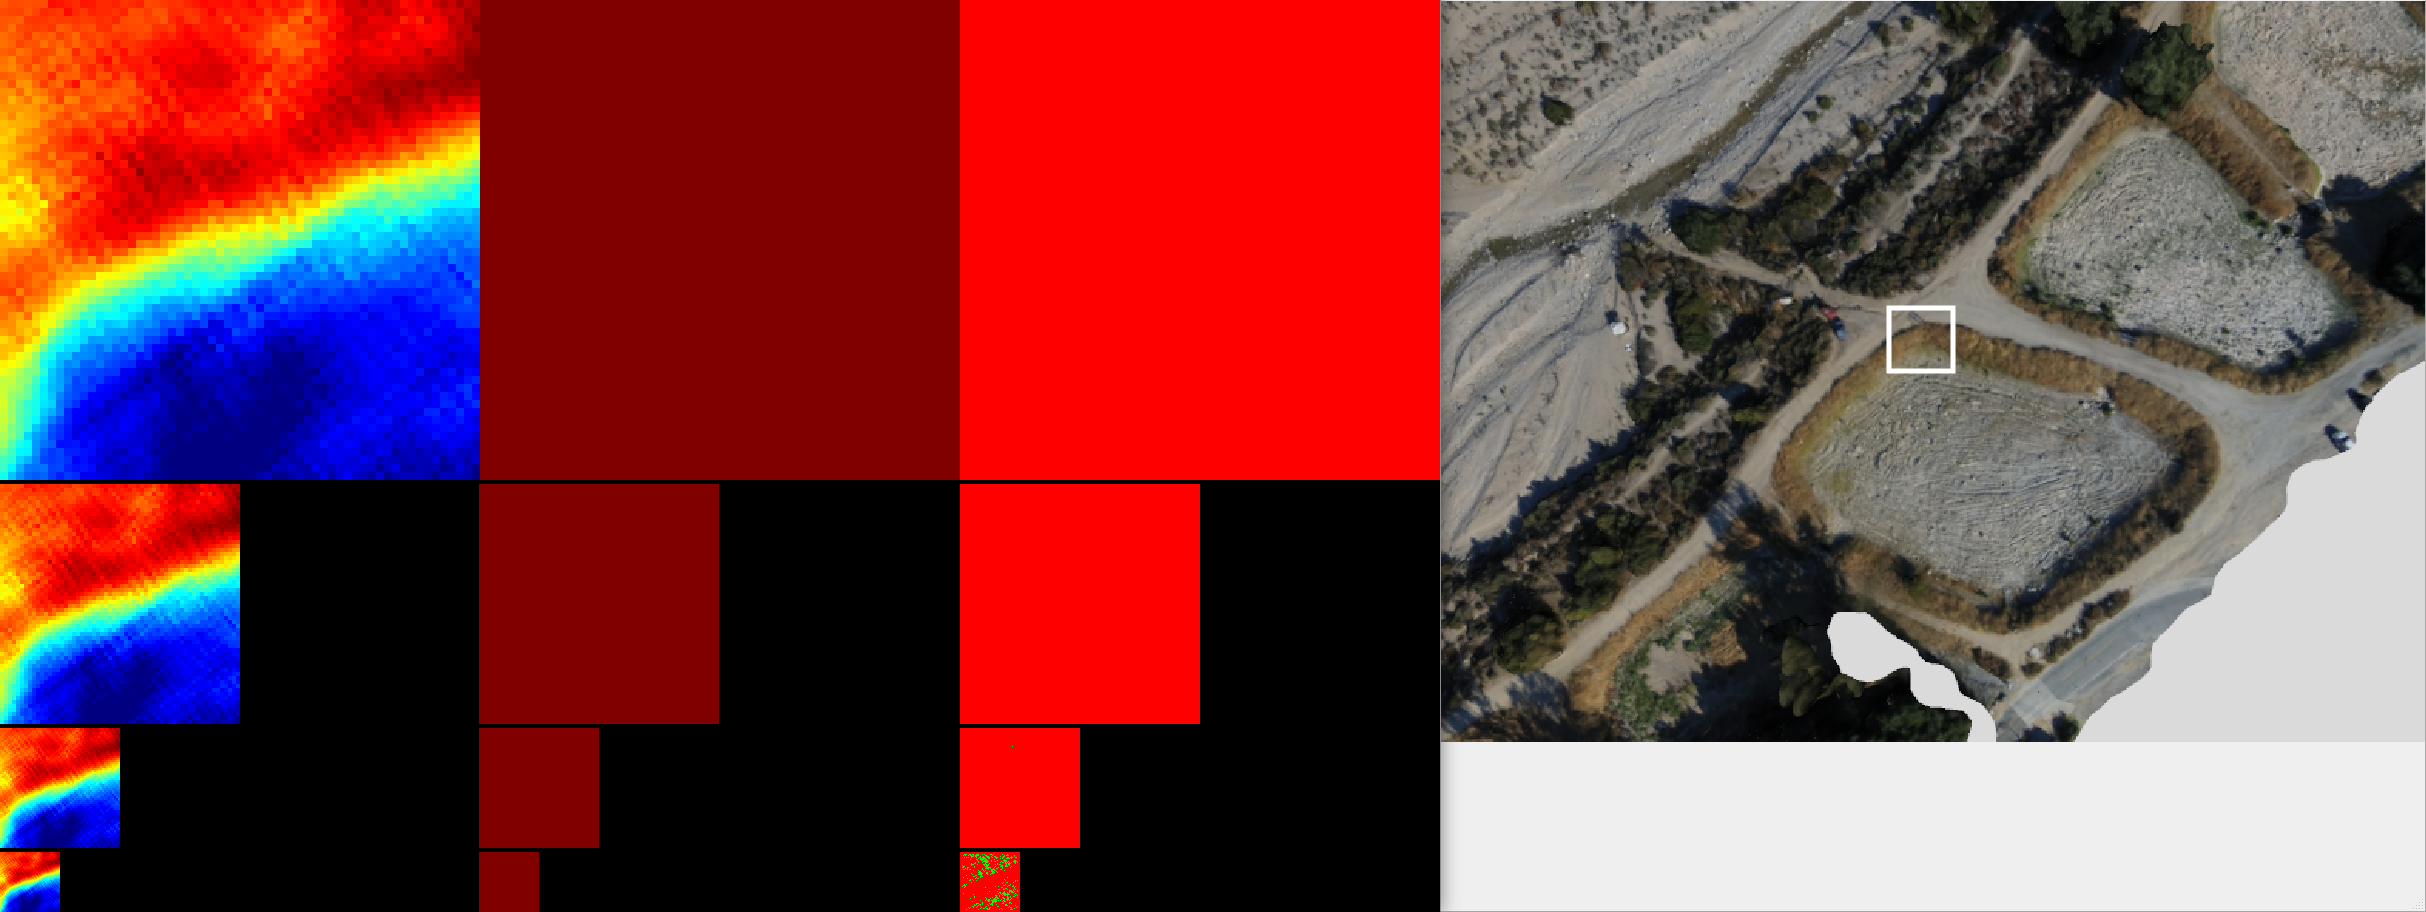
\includegraphics[scale=0.14]{images/evaluation/LSD_center_usage.png}
\caption{Comparison of the tracker camera image and the region of interest used by LSD}
\label{fig:LSD_center_usage}
\end{figure}

\subsection{Number of Layers}

Due to a fixed number of layers, the image points detected at high altitudes have a pixel footprint that exceeds that of a cell from the coarsest layer. Therefore, the point cloud input to LSD is sparse and leaves many cells empty. Empty cells prevent the detection of landing sites in the neighborhood. The smaller the coarsest layer's cell footprints, the stronger the effect. \cref{fig:lsd_2_layers_1} shows the LSD DEM before convergence when using 2 layers at 100 m altitude.

The lowest resolution layer has a fixed resolution of 0.05 m / cell. Considering the 4-fold division of a cell when moving to a higher resolution layer, the resolution at the top level is 0.2 m / cell. On the other hand, at 100 m altitude with the camera parameters introduced in \cref{sec:stereo_methodology}, the tracker camera's pixel footprint is 0.363 m/px. 

\begin{figure}[h]
\centering

\includegraphics[scale=0.24]{images/evaluation/2_layers_1.png}
\caption{LSD DEM at 100 m right after initialization with only 2 layers}
\label{fig:lsd_2_layers_1}
\end{figure}

After a while, the map is filled with further measurements as shown in \cref{fig:lsd_2_layers_2}.


\begin{figure}[h]
\centering
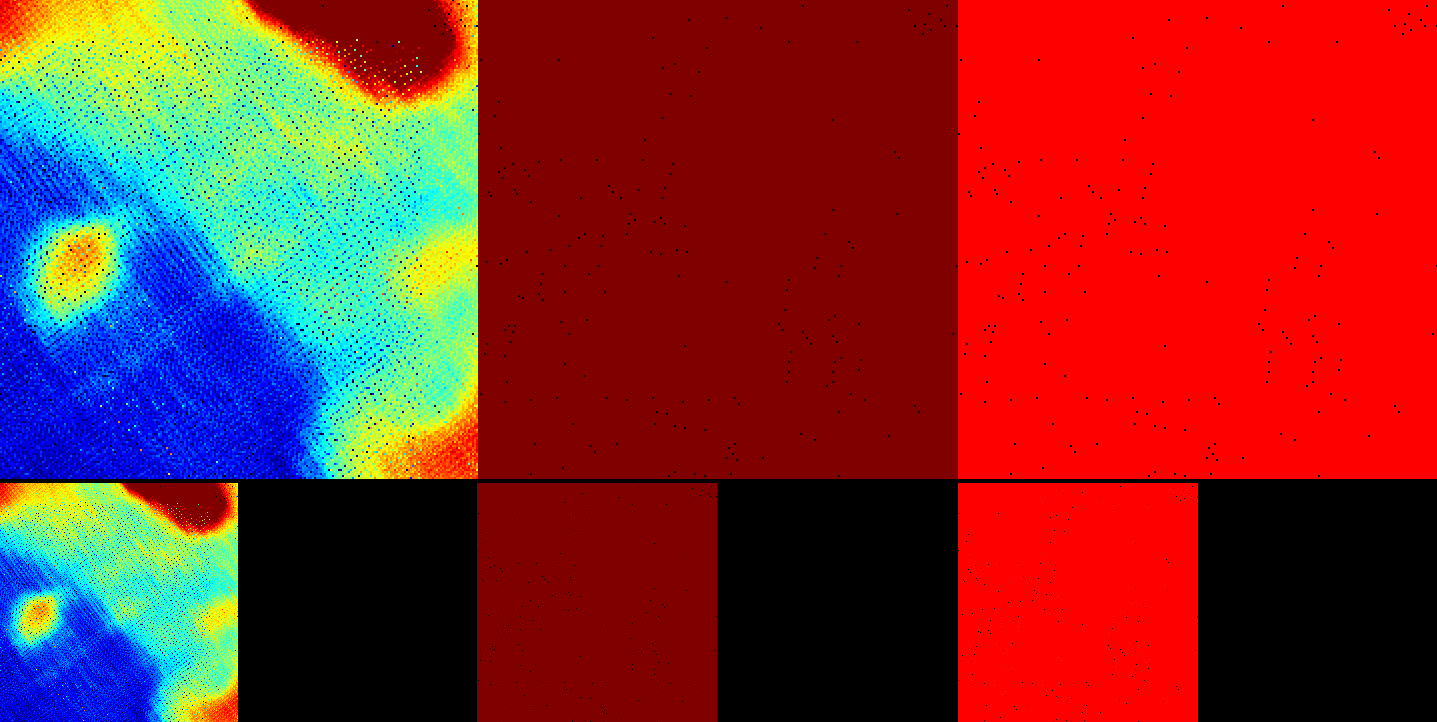
\includegraphics[scale=0.24]{images/evaluation/2_layers_2.png}
\caption{DEM at 100 m with 2 layers after some conversion time}
\label{fig:lsd_2_layers_2}
\end{figure}

\clearpage%HERE

However, due to the map movement mentioned in \cref{subsec:sfm_insufficiencies}, most of the DEM is erased before the DEM converges sufficiently.This is shown in \cref{fig:lsd_2_layers_3}. 

\begin{figure}[h]
\centering
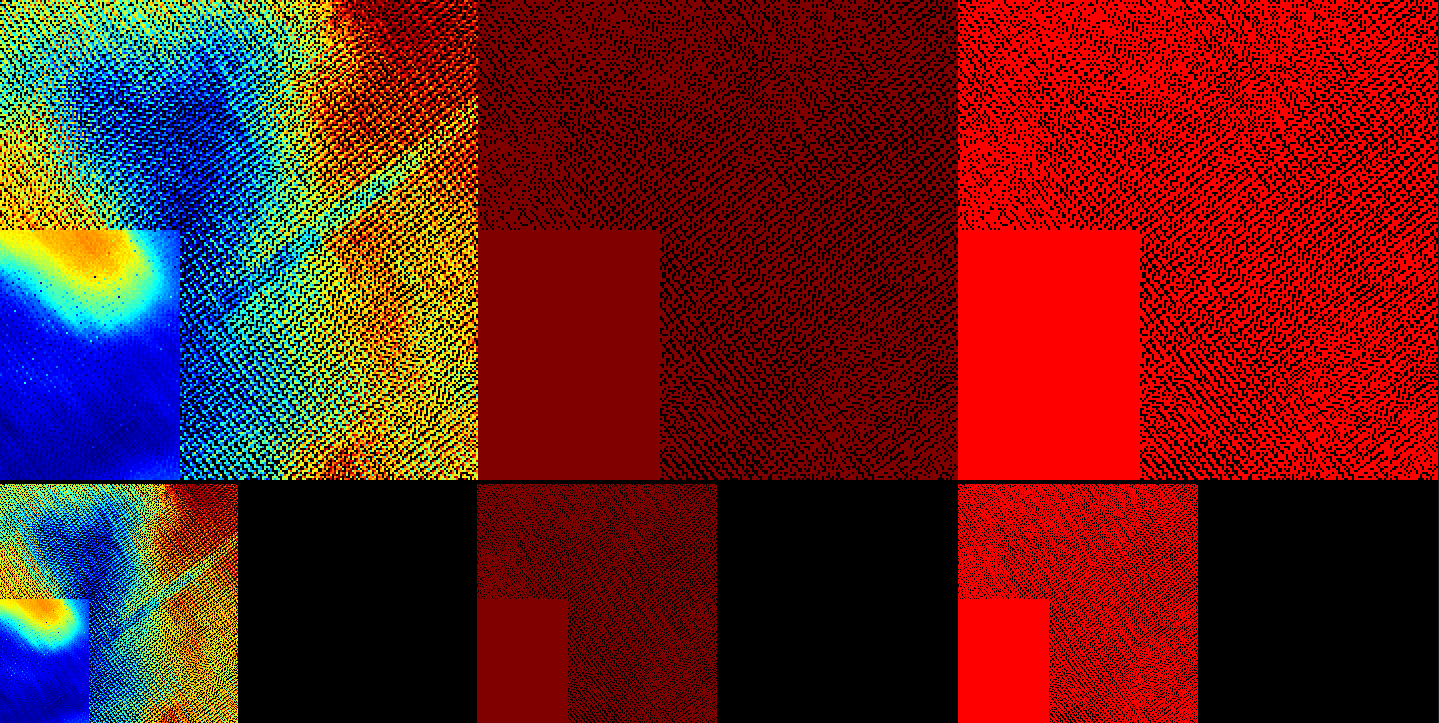
\includegraphics[scale=0.24]{images/evaluation/2_layers_3.png}
\caption{DEM at 100 m with 2 layers after map movement}
\label{fig:lsd_2_layers_3}
\end{figure}

A remedy for this is the usage of more layers, resulting in a decreased resolution at the coarsest layer. This way, the discrepancy between the footprints of the incoming points and the cells available is not as big, and as a result, the DEM is less sparse. It has to be noted, however, that using more layers leads to more computational overhead. An example LSD image shortly after initialization with 4 layers is shown in \cref{fig:lsd_4_layers_1}.

\begin{figure}[h]
\centering
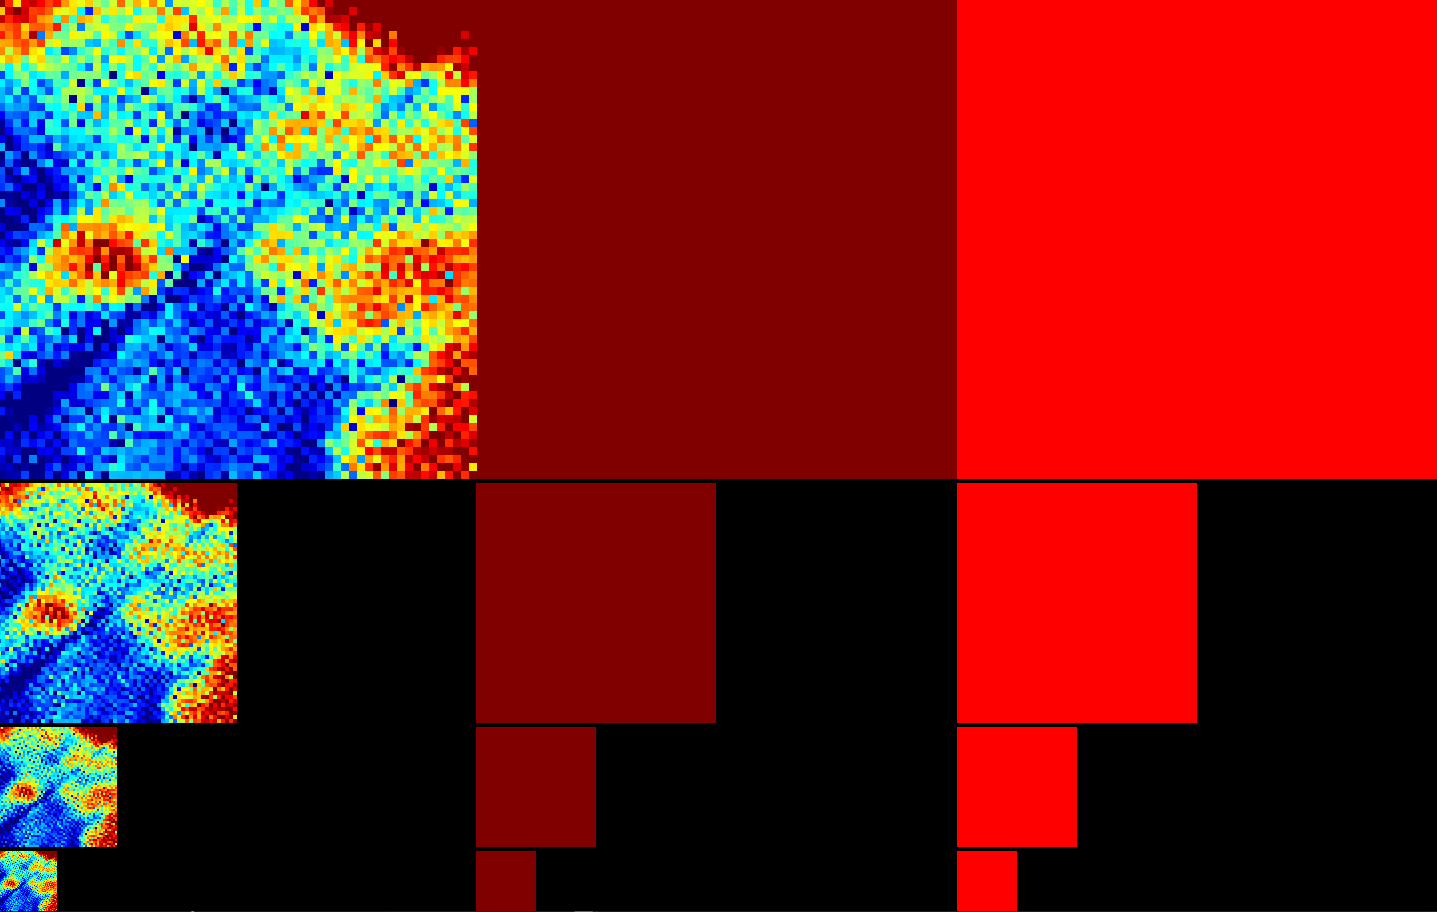
\includegraphics[scale=0.24]{images/evaluation/4_layers_1.png}
\caption{LSD DEM at 100 m with 4 layers}
\label{fig:lsd_4_layers_1}
\end{figure}

Note that more layers lead to a stronger pooling effect at the highest resolution layers. In other words, the sparsity of the DEM when using LSD with fewer layers is counteracted by the enhanced pooling of further layers, leading to a high-resolution layer filled with the same coarse information present at lower layers. Due to the incoming point cloud's large point footprint, there is no higher-resolution information to be had. Therefore, resolving the sparse maps with coarse information does not denote a loss of information. At high altitudes, we want to find areas with promising landing sites. These don't have to be perfect landing sites themselves yet and serve more as a signifier for later refinement. Thus, using lower-resolution information is perfectly nominal.

For a visual side by side comparison when using 2, 3, or 4 layers, see \cref{sec:layers}.

\section{Experimental Setup}\label{sec:exp_setup}

The pipeline was tested by repeatedly flying a mission with randomized initial conditions. On each setup, 100 flights were performed, and each flight was given a maximum of 10 minutes before the next iteration commenced.
\subsection{Simulated Terrain}\label{subsec:terrain}
The performed experiments were flown on the following two maps:
\begin{itemize}
    \item Arroyo Map - Map from the Arroyo Seco area outside the East entrance of the Jet Propulsion Laboratory. Predominantly used map during development
    \begin{figure}[h]
        \centering
        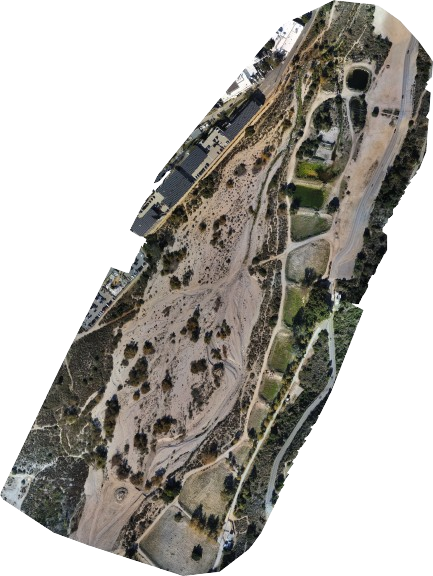
\includegraphics[scale=0.5]{images/evaluation/arroyo.png}
        \caption{Map of the Arroyo Seco area outside the Jet Propulsion Laboratory}
    \end{figure}
    \clearpage%HERE
    \begin{figure}[h]
        \centering
        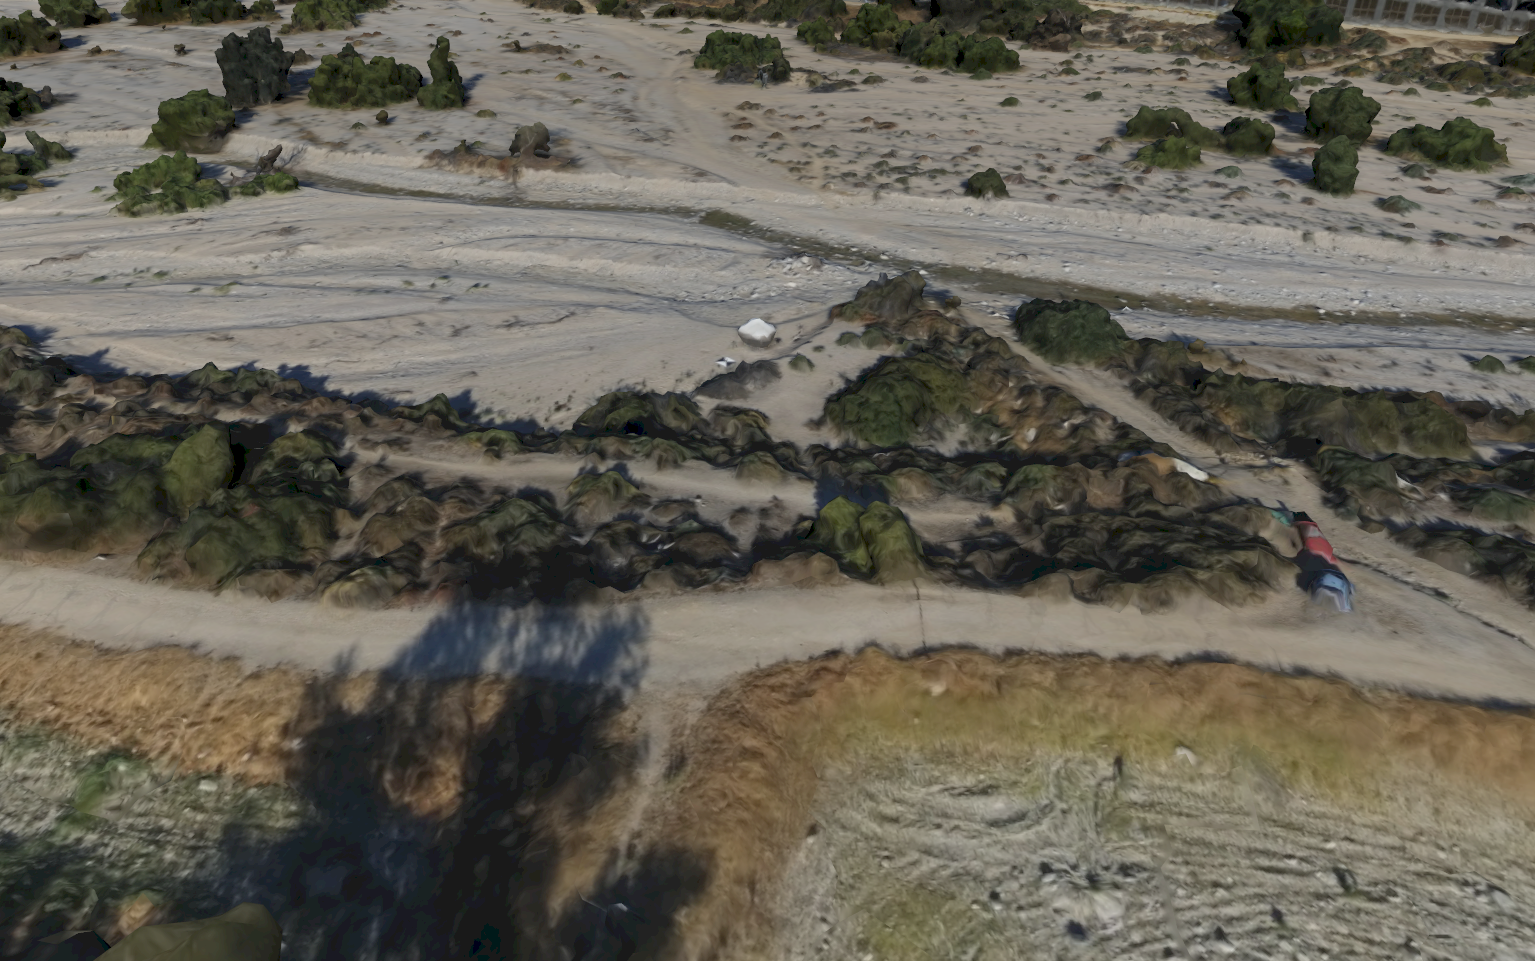
\includegraphics[scale=0.20]{images/evaluation/arroyo_map.png}
        \caption{Close Up of the Arroyo Map}
        \label{fig:sim_view_arroyo}
    \end{figure}
    \item Rough Test Map - A controlled environment designed to prevent LSD from detecting any landing site unless a landing platform is specifically spawned. It was created using Blender and applying white noise perturbations to the elevation of a plane. 
    \begin{figure}[h]
        \centering
        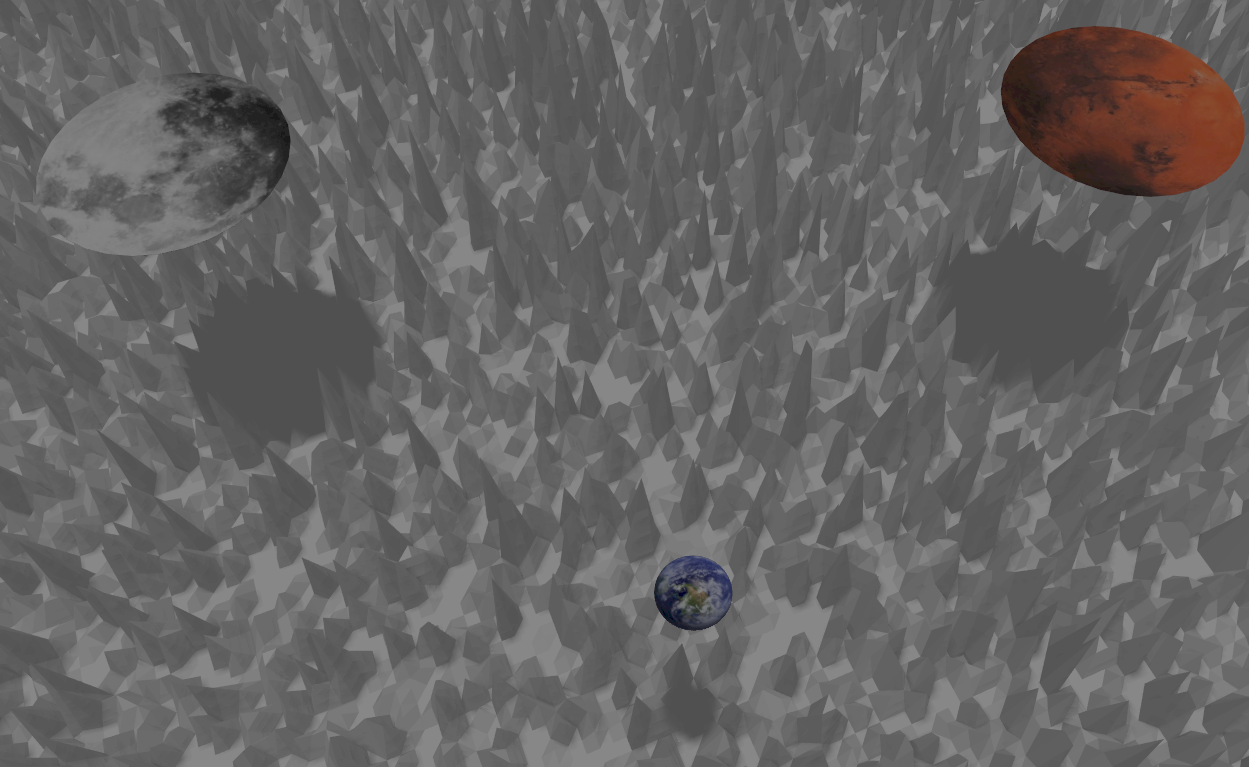
\includegraphics[scale=0.27]{images/evaluation/rough_test_map.png}
        \caption{Synthetically created, hazardous map with no landing sites apart from inserted landing platforms.}
    \end{figure}
    \begin{figure}[h]
        \centering
        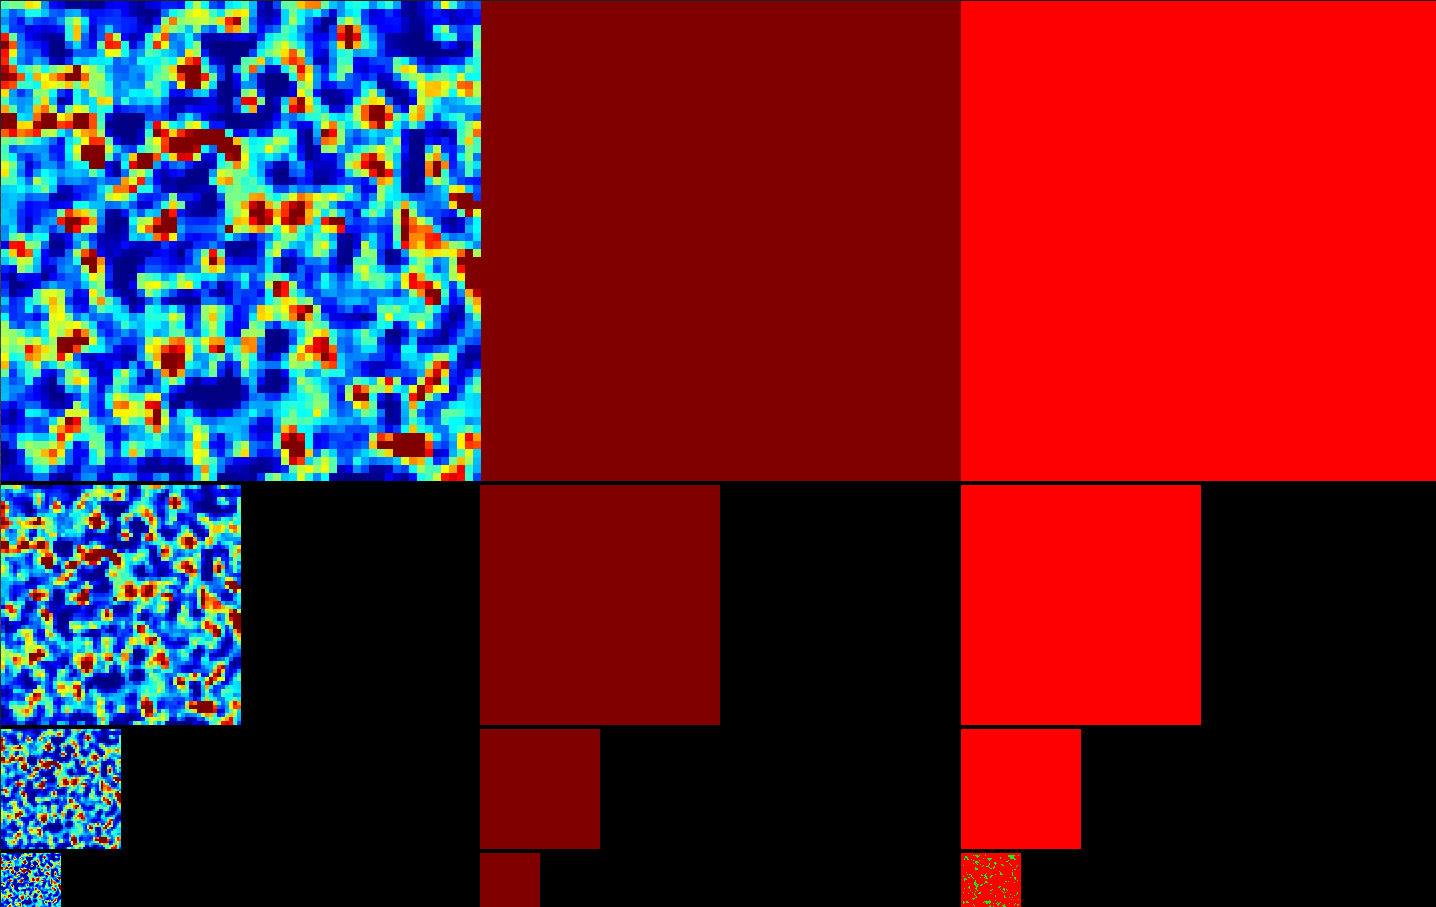
\includegraphics[scale=0.25]{images/evaluation/rough_map_LSD.png}
        \caption{LSD debug output shown of the plain rough environment}
    \end{figure}
    \begin{figure}[h]
        \centering
        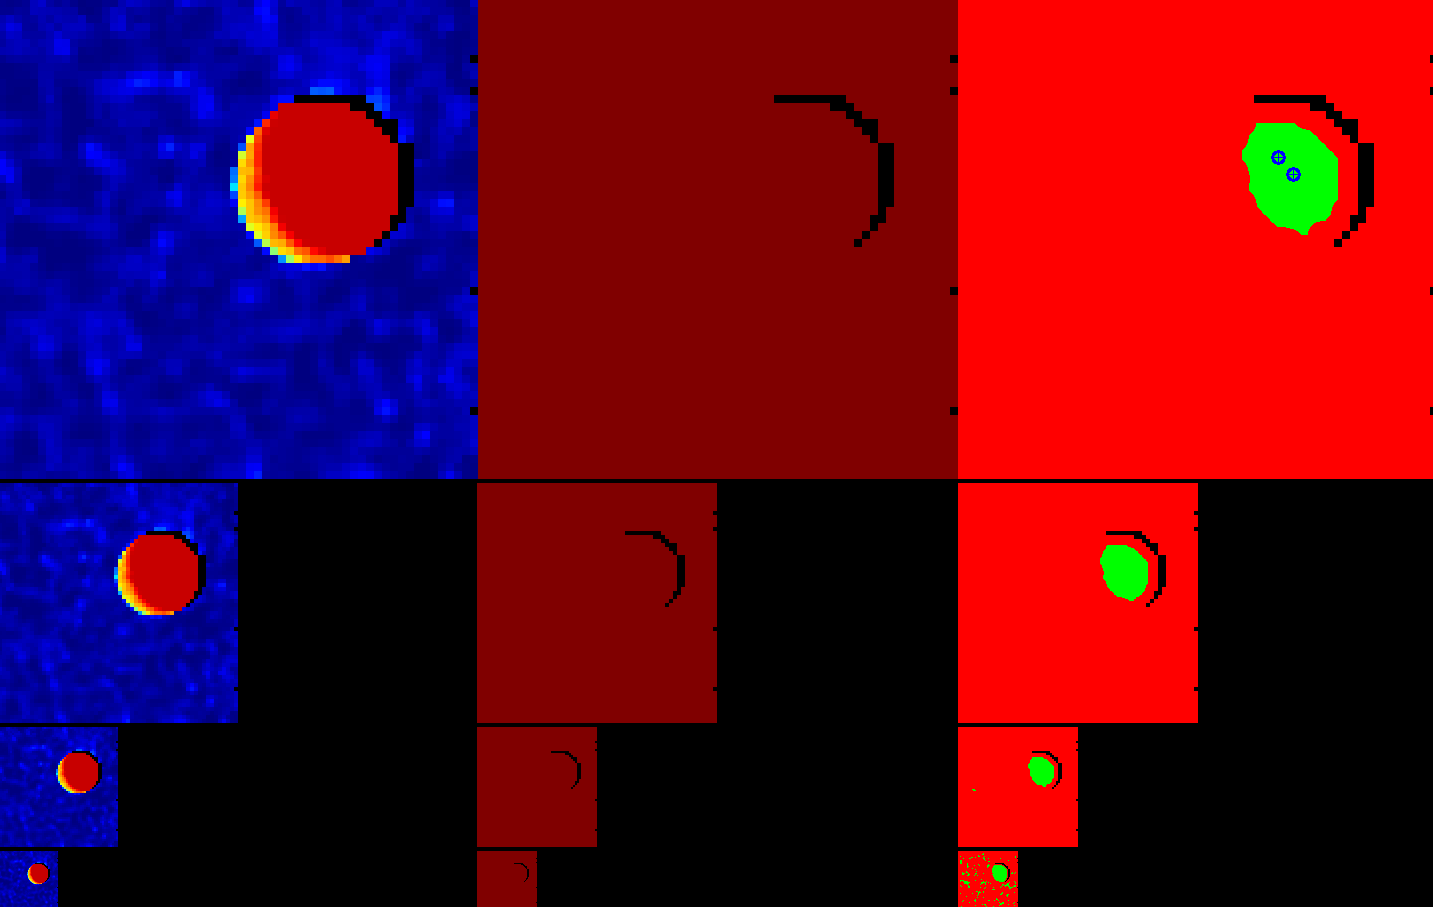
\includegraphics[scale=0.25]{images/evaluation/rough_map_LSD_platform.png}
        \caption{LSD debug image of the rough control map with spawned landing platforms}
        \label{fig:rough_map_platform}
    \end{figure}
\end{itemize}
\clearpage%HERE
\subsection{Drone Spawn}
The drone was either spawned repeatedly from a default location on the ground (The start location from when the actual field tests were performed) or from a random location. For a simple way of avoiding terrain collisions, the drone was spawned on a randomly positioned disk at 40 m altitude. The start disk's size was only 0.5 m in diameter which prevented it from being considered too good of a landing site by LSD. This is important because the platform implicitly gains quality since it is located higher up than the terrain, leading to a lower distance to the drone when flying at mission altitude.
\begin{figure}[h]
    \centering
    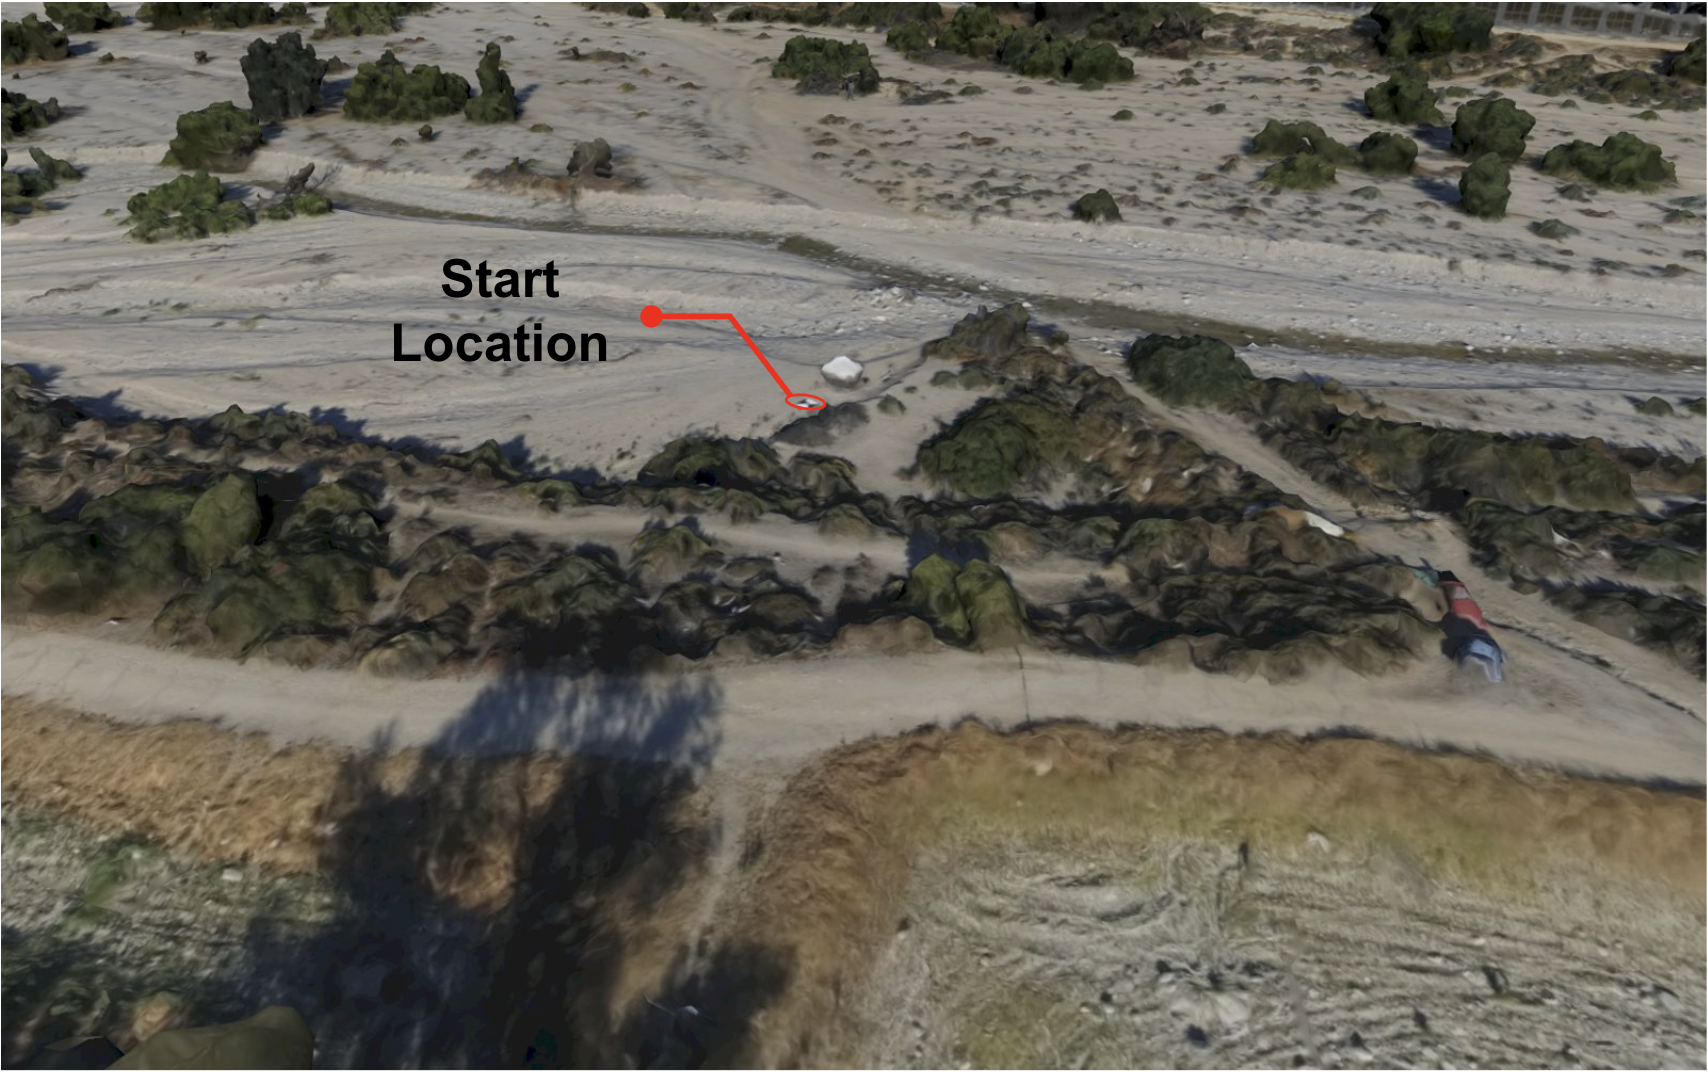
\includegraphics[scale=0.42]{images/evaluation/arroyo_with_start.png}
    \caption{Arroyo Map with Fixed Start Position}
    \label{fig:fixed_start}
\end{figure}
\begin{figure}[h]
    \centering
    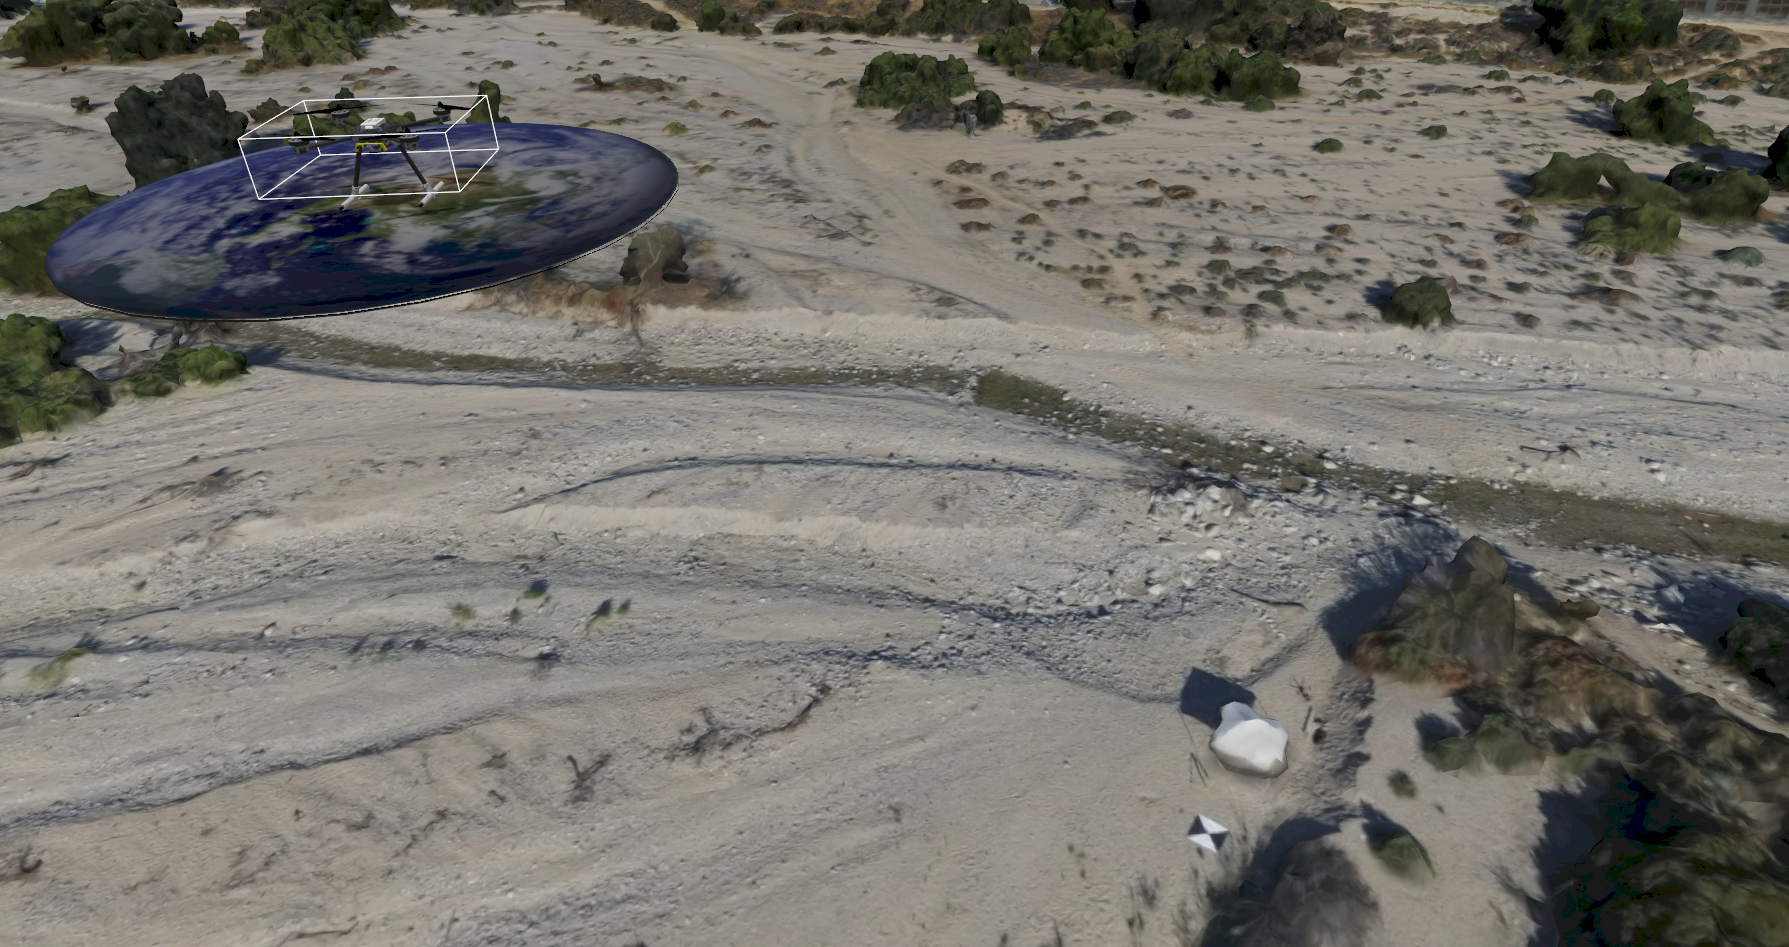
\includegraphics[scale=0.2]{images/evaluation/arroyo_with_platform.png}
    \caption{Arroyo map with randomly positioned spawn platform}
    \label{fig:random_start}
\end{figure}
\clearpage %HERE

\subsection{Depth Source}
As mentioned in \cref{subsec:sfm_insufficiencies}, at the time of this work, SFM was very fragile as an individual module. Because of this and to evaluate the landing pipeline instead of the depth generation module, ground truth depth was used above the verification altitude. For the sake of completeness, however, an SFM run is also shown in the end. Regardless of whether ground truth or SFM was used, the verification at low altitudes was always performed using the stereo camera depth node.

Note that at the rough map introduced in \cref{subsec:terrain}, no texture is projected onto the terrain. Therefore, on this map, ground truth was used exclusively.

\subsection{Success Conditions}
Two main metrics were considered to determine whether a flight was successful. First, it was checked whether the landing action in autonomy was initiated (this happens only after the landing site selection and verification are both successful).
Secondly, a rosbag was recorded for each flight. To infer the safety of the rotorcraft, the bag was analyzed to check whether either the roll or pitch value exceeded the crash threshold. In practice, a threshold of 1.2 radians or shortly below 70 degrees proved to be an accurate decision boundary to detect a drone crash.

\subsubsection{Home Landings}
Landing at the home position defines the behavior when the drone does not navigate towards a landing site but instead uses the stored takeoff coordinates to navigate to the spawn location to land. This happens when no landing sites exist to be chosen.

This occurs in two scenarios:
\begin{itemize}
    \item Few landing sites were detected yet failed verification and were therefore banned. Thereafter, no landing sites remained.
    \item No landing sites were detected in the first place. 

    This can happen because of two reasons:
    \begin{itemize}
        \item The overflown terrain simply does not have a single landing site of decent quality. (see the rough map introduced in \cref{sec:exp_setup})
        \item The landing site detection algorithm failed to detect landing sites.
    \end{itemize}
\end{itemize}
    
    In both scenarios, going home is the desired behavior. However, if LSD does not detect landing sites where good candidates should be found, the run cannot be counted as a success, regardless of whether the drone landed safely after taking off.

    For instance, looking at the Arroyo map shown in \cref{fig:sim_view_arroyo} and running numerous simulated flights on the terrain, it is clear that sufficient landing sites should be found on this map. Therefore, landing at home when flying on the Arroyo map indicates a landing site pipeline issue.
\subsubsection{Off Board Mode connection Issues}
Occasionally, connection failures between the PX4 flight controller and the autonomy occurred, leading to the deactivation of the off-board mode and, therefore, the loss of control of the autonomy over the rotorcraft. These issues arose most likely because the MAVROS connection in between failed to send a necessary repeated heartbeat, and thus, the connection was intercepted.

Self-evidently, this did not result in a guaranteed successful landing and was not counted as such. However, as these connection issues did not occur due to insufficiencies in the pipeline presented in this work, they were not considered failures of the pipeline either. 

Therefore, to conclude the listing of the possible success states:

\begin{itemize}
    \item Successful: The drone initiated the landing and did not fall over throughout the whole flight.
    \item Connection loss: The autonomy lost the connection to the flight controller, and therefore, no information can be gathered about this flight and the landing behavior's performance.
    \item Crash: Either the roll or pitch angle of the drone exceeded the predetermined threshold of 70 degrees. This is a definite failure of the pipeline.
    \item Home landing: The drone did not settle at a perceived landing site and returned to the home position instead. On a map with sufficient landing opportunities, this indicates a failure. When actually not traversing terrain with valid landing sites, as was often the case for the rough terrain shown in \cref{subsec:rough_map_rw}, landing home is the desired behavior.
\end{itemize}


\subsection{Visual Analysis}
To further analyze the randomized flights in a bit more detail, visual landing attempt projections are used. Such an analysis image is shown in \cref{fig:landing_attempts_dummy}.

The green points indicate successful verifications, which lead to the initiation of the landing action shortly afterward. (If no rotation above a failure threshold was detected, this is considered a successful landing.) 

The yellow points are landing attempts, where a chosen landing site was not verified and thus banned from further consideration. It is crucial to note that not being able to verify a landing site is no issue at all. Landing sites detected at high altitudes merely provide a preliminary indication of potential landing zones. The subsequent phase, responsible for verifying these sites, yields the refined final landing site knowledge used for landing. So selecting a landing site at a high altitude, not being able to verify it, and subsequently choosing a nearby landing site might even be called the most sustainable chain of actions in the pursuit of autonomous landing.

Blue points indicate successful landings achieved through the trigger of the landing-at-home action. As previously mentioned, When flying on a map with obvious landing opportunities, triggering the landing-at-home action indicates an issue with the landing site detection mechanism.

Lastly, red dots indicate landing sites that were detected during a flight that was disrupted by a connection issue.

If multiple landing attempts are made, connection lines are drawn between the failed attempts and the final landing, indicating which subsequent sites were chosen.

It has to be noted that these plots were generated using non-orthographic background images, and the actual landings took place at locations slightly closer to the image center.

\begin{figure}[h]
    \begin{center}
        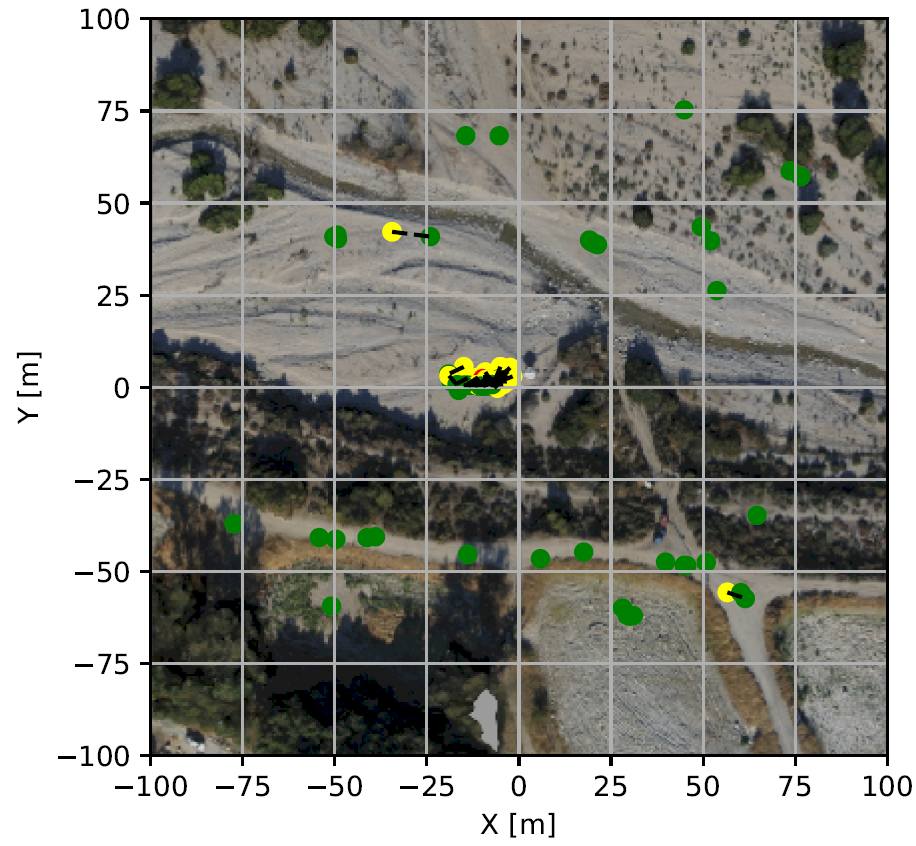
\includegraphics[scale=0.5]{images/evaluation/landings_random_WP_GT.png}
        \caption{Landing Attempt dummy image - Green: successful landing, Yellow: verification failure, Blue: landing at home position}
        \label{fig:landing_attempts_dummy}
    \end{center}
\end{figure}

As the created points are rather large, \cref{fig:Arroyo_BG} shows the empty background image for reference.

\begin{figure}[h]
\centering
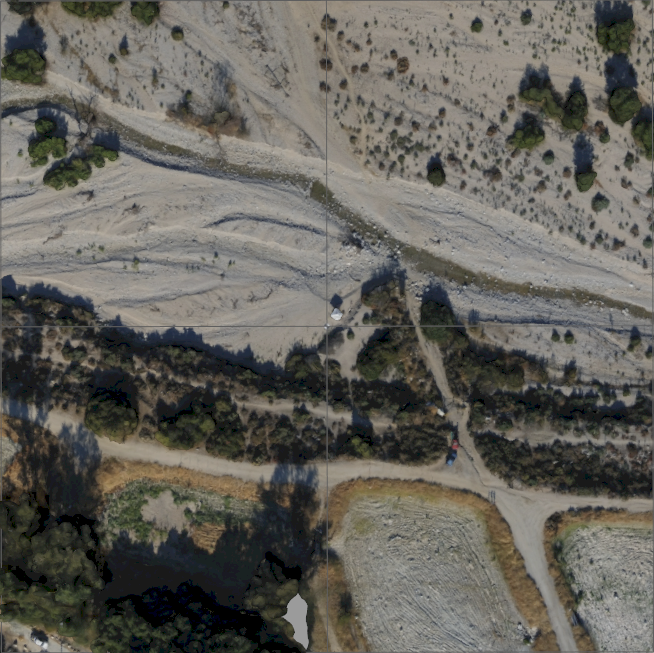
\includegraphics[scale=0.4]{images/evaluation/high_100m_arroyo_grid.png}
\caption{Non-orthographic Arroyo background image for visual evaluation of the test flights}
\label{fig:Arroyo_BG}
\end{figure}
\clearpage%HERE

\section{Test Flights}\label{sec:test_flights}

The following tests were performed. Each test consisted of 100 flights simulated in Gazebo.

\subsection{Arroyo - Randomized Waypoints}\label{subsec:eval_rand_wp}

When starting 100 times from the fixed position indicated in \cref{fig:fixed_start} and flying to random mission waypoints at 100 m altitude in a 70x70m vicinity on the Arroyo map, the following results were achieved:

\begin{table}[h]
    \begin{center}
     \caption{Results with fixed takeoff and random waypoint: Con. Loss stands for connection loss of the off-board mode.}\vspace{1ex}
     \label{tab:result_random_waypoint}
     \begin{tabular}{|c|c|c|c|c|}
     \hline
     \# Flights & \# Successes & \# Con. Loss & \# Crashes & \# Home Landing\\ \hline \hline
     100 & 93 & 7 & 0 & 0 \\
     \hline
     \end{tabular}
    \end{center}
    \end{table}

    The landing attempt numerics are shown here:

    \begin{table}[h]
        \begin{center}
         \caption{Landing attempts with fixed takeoff and random waypoint}\vspace{1ex}
         \label{tab:land_nums_random_waypoint}
         \begin{tabular}{|c|c|c|c|}
         \hline
         \# Flights & \# Landing on first attempt & \# 2 attempts & \# 3 attempts\\ \hline \hline
         93 & 58 & 33 & 2 \\
         \hline
         \end{tabular}
        \end{center}
    \end{table}

    \begin{figure}[h]
        \begin{center}
            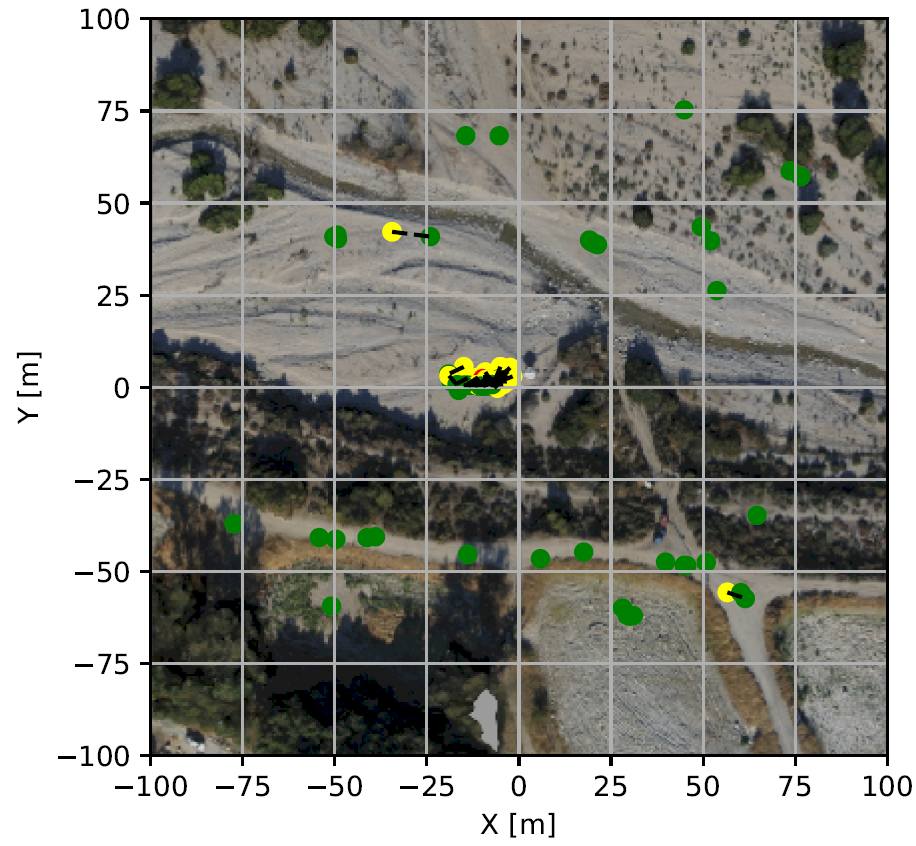
\includegraphics[scale=0.5]{images/evaluation/landings_random_WP_GT.png}
            \caption{Landing Attempts - Green: successful landing, Yellow: verification failure, Blue: landing at home position}
            \label{fig:landing_attempts_random_WP}
        \end{center}
    \end{figure}

    \subsubsection{Numeric Discussion}
    \cref{tab:result_random_waypoint} shows the numeric outcome of the flights. 7 timeouts occurred, but each performed flight by the autonomy was a success, landing safely and controlled. No home landings were necessary, which, as described above, indicates a very robust LSD performance. A high number of flights where two landing site verification attempts were performed is also well within acceptable boundaries because the first landing site might as well be used as an indicator to draw the drone closer to an area where high-quality sites can be detected using the stereo camera. Twice it was the case that 3 landing attempts were needed.

    \subsubsection{Visual Discussion}
    Let's consider the landing image \ref{fig:landing_attempts_random_WP}. The final landing sites indicated in green span exclusively decent landing areas. The verification attempts that fell short are indicated with yellow and annotated by a line connection to the successful attempt thereafter. Subsequent landing sites were always detected short distances away from failed candidates which is exactly the correct behavior in order not to lose time pursuing a far away follow-up landing site. As indicated in \cref{subsec:heuristics}, this is thanks to the verification altitude, which incentivizes the selection of other landing sites detected at the current verification altitude. Lastly, landing attempts performed before losing the connection to the flight controller are indicated in red. Note, an example log file of a flight which lost connection to the flight controller is shown in \cref{sec:specific_runs}.
    
    The last thing to mention is the clustering of the landing sites around the takeoff location. The reason for this is twofold:
    \begin{itemize}
        \item Quality: 
        
        The takeoff position in the simulation was chosen to be at the same location where the field tests were started in the real world. It was chosen exactly because of its even and smooth characteristics. Therefore, it is no surprise that many landing sites were detected around that location. 
        \item OMG Conversion: 
        
        During ascent, when using either stereo or ground truth depth, the same area is perceived repeatedly. This leads to a convergence of OMG certainty in the map aggregation step of LSD. As landing sites have a higher chance of being detected on terrain with low uncertainty, this converged takeoff area is most likely selected repeatedly and sent to the autonomy until it leaves the rolling buffer map. 
        
        Note: the autonomy framework accounts for repeated detection of the same landing site. LSD however does not. Therefore, in such a case where the same terrain has been viewed for a long period, it is possible for the exact same landing site proposals to be sent to the autonomy repeatedly.
    \end{itemize}

    This test is a very clear demonstration of the applied chosen heuristics. The best landing site detected is very likely one that is detected at the takeoff position. Around this clustering of landings, there is a notable space where no attempts have been performed. This can be attributed to the competing motives of the landing site selection. The quality of the landing site defines the autonomy's choice until the drone's distance to that landing site is too big, and a closer one is chosen. 

% \subsection{Arroyo - Farther Randomized Waypoints}\label{subsec:far_eval_rand_wp}
% To test the pipeline's proclivity towards the selection of landing sites near the spawn point, the same experiment is run again whilst making sure the mission waypoints are at least 40 m away from the spawn location.
% \begin{table}[h]
%     \begin{center}
%      \caption{Results with fixed takeoff and random waypoints at least 40 m from the spawn}\vspace{1ex}
%      \label{tab:result_far_random_waypoint}
%      \begin{tabular}{|c|c|c|c|c|}
%      \hline
%      \# Flights & \# Successes & \# Timeouts & \# Crashes & \# Home Landing\\ \hline \hline
%      100 & 99 & 1 & 0 & 0 \\
%      \hline%TODO: fill with real values
%      \end{tabular}
%     \end{center}
%     \end{table}
%     The landing attempt numerics are shown here:
%     \begin{table}[h]
%         \begin{center}
%          \caption{Landing attempts with fixed takeoff and random waypoints at least 40 m from the spawn}\vspace{1ex}
%          \label{tab:land_nums_far_random_waypoint}
%          \begin{tabular}{|c|c|c|c|}
%          \hline
%          \# Flights & \# Landing on first attempt & \# 2 attempts & \# 3 attempts\\ \hline \hline%TODO: replace
%          100 & 48 & 45 & 7 \\
%          \hline
%          \end{tabular}
%         \end{center}
%     \end{table}
%     \begin{figure}[h]
%         \begin{center}
%             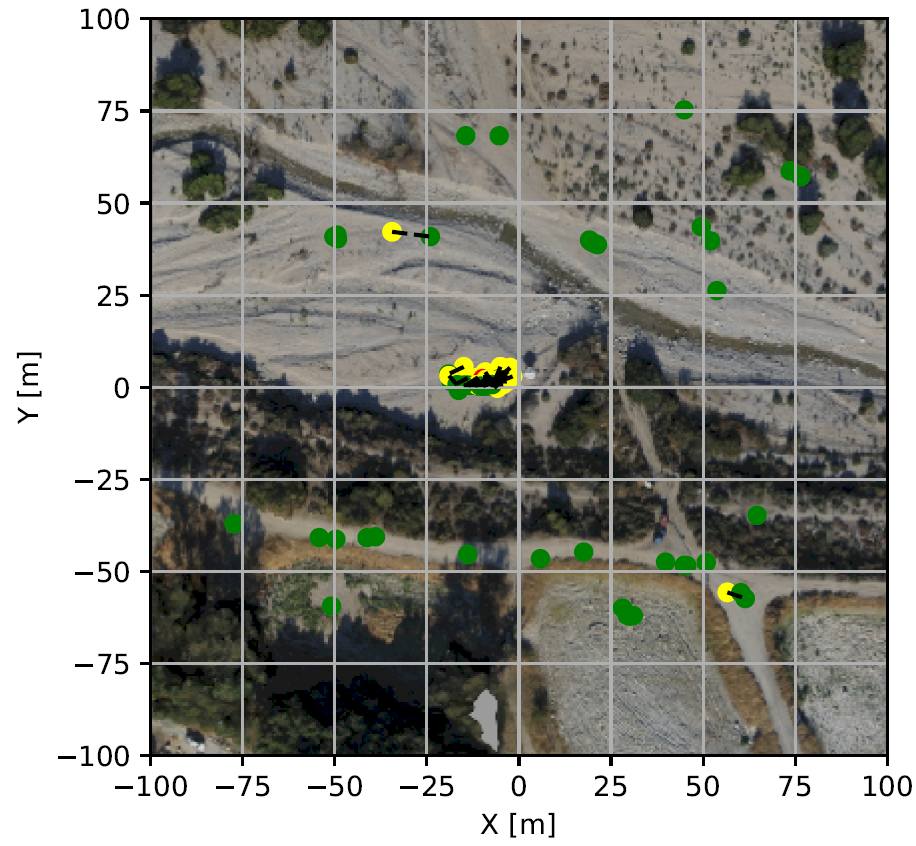
\includegraphics[scale=0.5]{images/evaluation/landings_random_WP_GT.png}
%             \caption{Landing Attempts - Green: successful landing, Yellow: verification failure, Blue: landing at home position}
%             \label{fig:landing_attempts_far_random_WP}
%         \end{center}%TODO: replace
%     \end{figure}
%     \subsubsection{Numeric Discussion}
% %TODO
%     \subsubsection{Visual Discussion}
% %TODO

\clearpage%HERE

\subsection{Arroyo - Randomized Takeoff and Waypoints}\label{subsec:compl_rand}

    In this set of test flights, randomized takeoff positions were used as shown in \cref{fig:random_start}. Missions were built using a randomized waypoint in a 70x70m surrounding.

    The numerical results look as follows:

    \begin{table}[h]
        \begin{center}
         \caption{Results with random takeoff location and random waypoint}\vspace{1ex}
         \label{tab:result_complete_rand}
         \begin{tabular}{|c|c|c|c|c|}
         \hline
         \# Flights & \# Successes & \# Con. Losses & \# Crashes & \# Home Landing\\ \hline \hline
         100 & 94 & 6 & 0 & 0 \\
         \hline
         \end{tabular}
        \end{center}
    \end{table}
    \begin{table}[h]
        \begin{center}
         \caption{Landing attempts with random takeoff and random waypoint}\vspace{1ex}
         \label{tab:land_nums_complete_rand}
         \begin{tabular}{|c|c|c|c|c|}
         \hline
         \# LS Landings & \# 1 attempt & \# 2 attempts & \# 3 attempts & \# 4 attempts\\ \hline \hline
         94 & 88 & 6 & 0 & 0 \\
         \hline
         \end{tabular}
        \end{center}
    \end{table}

    And the visual outcome is shown in \cref{fig:landing_attempts_complete_rand}.

    \begin{figure}[h!]
        \begin{center}
            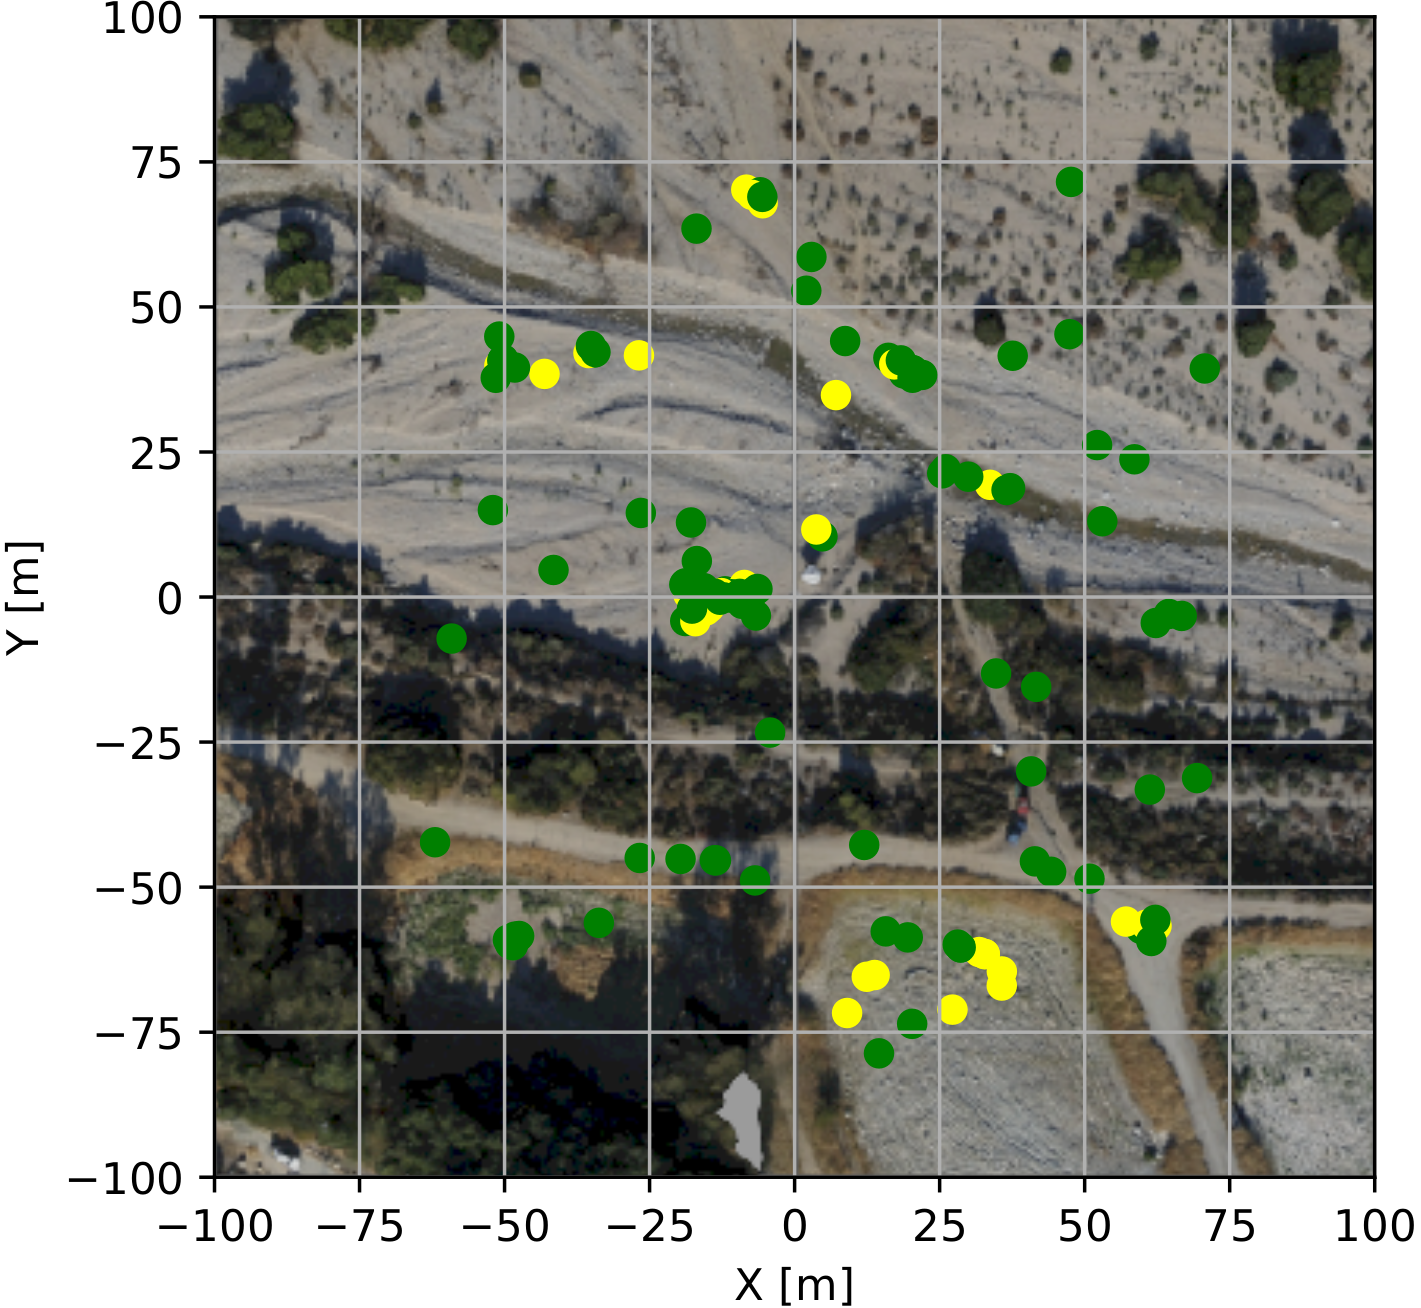
\includegraphics[scale=0.5]{images/evaluation/landings_complete_randomized_GT.png}
            \caption{Landing attempts with randomized drone spawn - Green: successful landing, Yellow: verification failure, Blue: landing at home position}
            \label{fig:landing_attempts_complete_rand}
        \end{center}
    \end{figure}

    \subsubsection{Numeric Discussion}
    6 timeouts occurred in this 100-flight experiment. Of the successful 94 runs, 88 landed at the very first attempt, and only 6 needed one more landing site. This is a pleasant outcome, which is, of course, correlated with the ground truth's high accuracy. Nevertheless, it has to be noted that multiple landing attempts at different sites are no indication of inferior performance. 

    The relatively high number of timeouts is undesirable, but as previously mentioned, it is not a fault of the presented pipeline and is therefore merely unfortunate but not worrying.


    \subsubsection{Visual Discussion}
    Compared to \cref{fig:landing_attempts_random_WP}, the landing attempts are more spread out over the map, and fewer landings were attempted at the takeoff position. This is the case because the random mission trajectories didn't always cover this area, and since the drone spawned at randomized locations, it did not spend the time during takeoff to repeatedly scan this plateau. Thus, the elevation map did not converge at that location leading to a smaller chance of landing sites being detected there. 
    
    As for the fixed spawn location, the second attempts were always at landing sites close to the false previous candidates. This is, of course, desirable to save time.

    Lastly, the selected landing sites were all at plausible locations. To verify this, consider the empty reference image shown in \cref{fig:Arroyo_BG}

\subsection{Rough Map - Mission Covering Platforms}\label{subsec:rough_coverage}
        \begin{figure}[h]
            \centering
            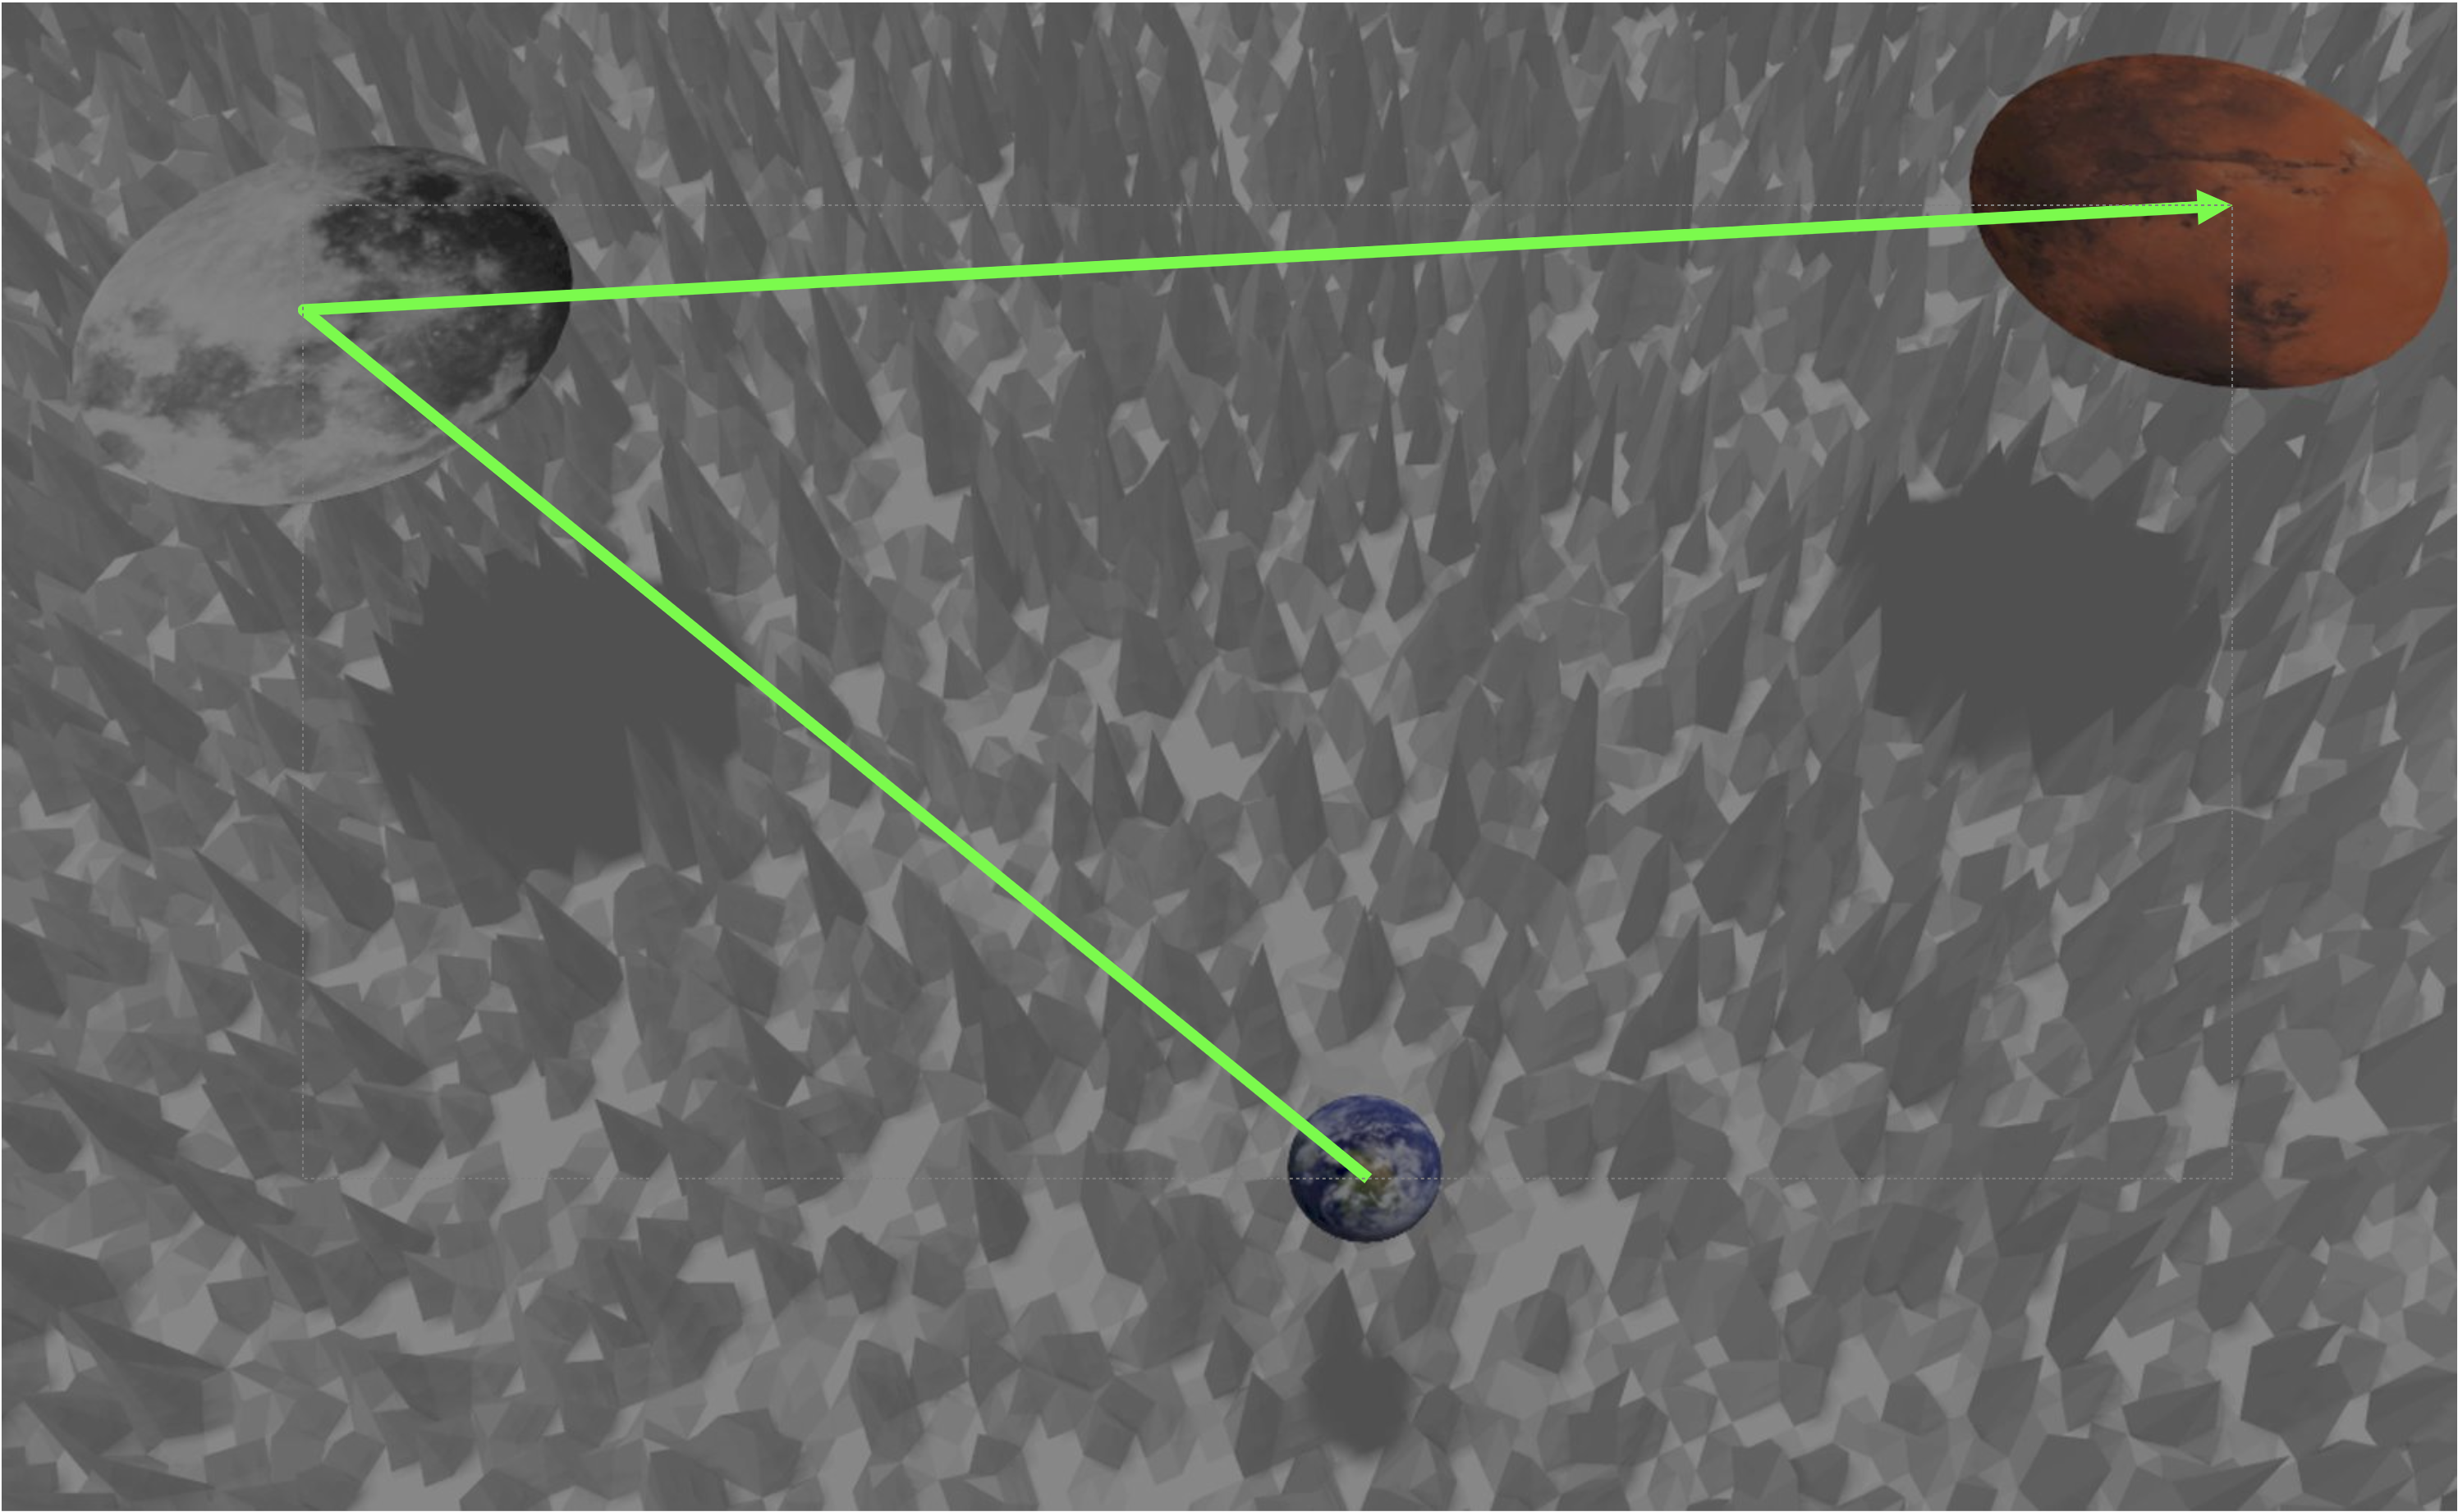
\includegraphics[scale=0.24]{images/evaluation/rough_over_platforms.png}
            \caption{Test flights on rough map with waypoints covering the landing sites}
            \label{fig:rough_covered}
        \end{figure}

        In this test, the drone flew a randomized two-waypoint pattern which always covered the synthetically added landing platforms. The idea behind this experiment was to eliminate other landing possibilities and test whether the approach at hand would be able to detect the controlled good landing sites.

        The numerical result thereof is displayed below:

        \begin{table}[h]
            \begin{center}
             \caption{Results - Rough map with platform coverage}\vspace{1ex}
             \label{tab:result_rough_covered}
             \begin{tabular}{|c|c|c|c|c|}
             \hline
             \# Flights & \# Successes & \# Con. Losses & \# Crashes & \# Home Landing\\ \hline \hline
             100 & 99 & 1 & 0 & 0 \\
             \hline
             \end{tabular}
            \end{center}
        \end{table}

        \begin{table}[h]
            \begin{center}
             \caption{Landing attempts rough map with platform covering mission}\vspace{1ex}
             \label{tab:land_nums_rough_coverage}
             \begin{tabular}{|c|c|c|c|}
             \hline
             \# LS landing & \# Landing on first attempt & \# 2 attempts & \# 3 attempts\\ \hline \hline
             99 & 98 & 1 & 0 \\
             \hline
             \end{tabular}
            \end{center}
        \end{table}

        \begin{figure}[h]
        \centering
        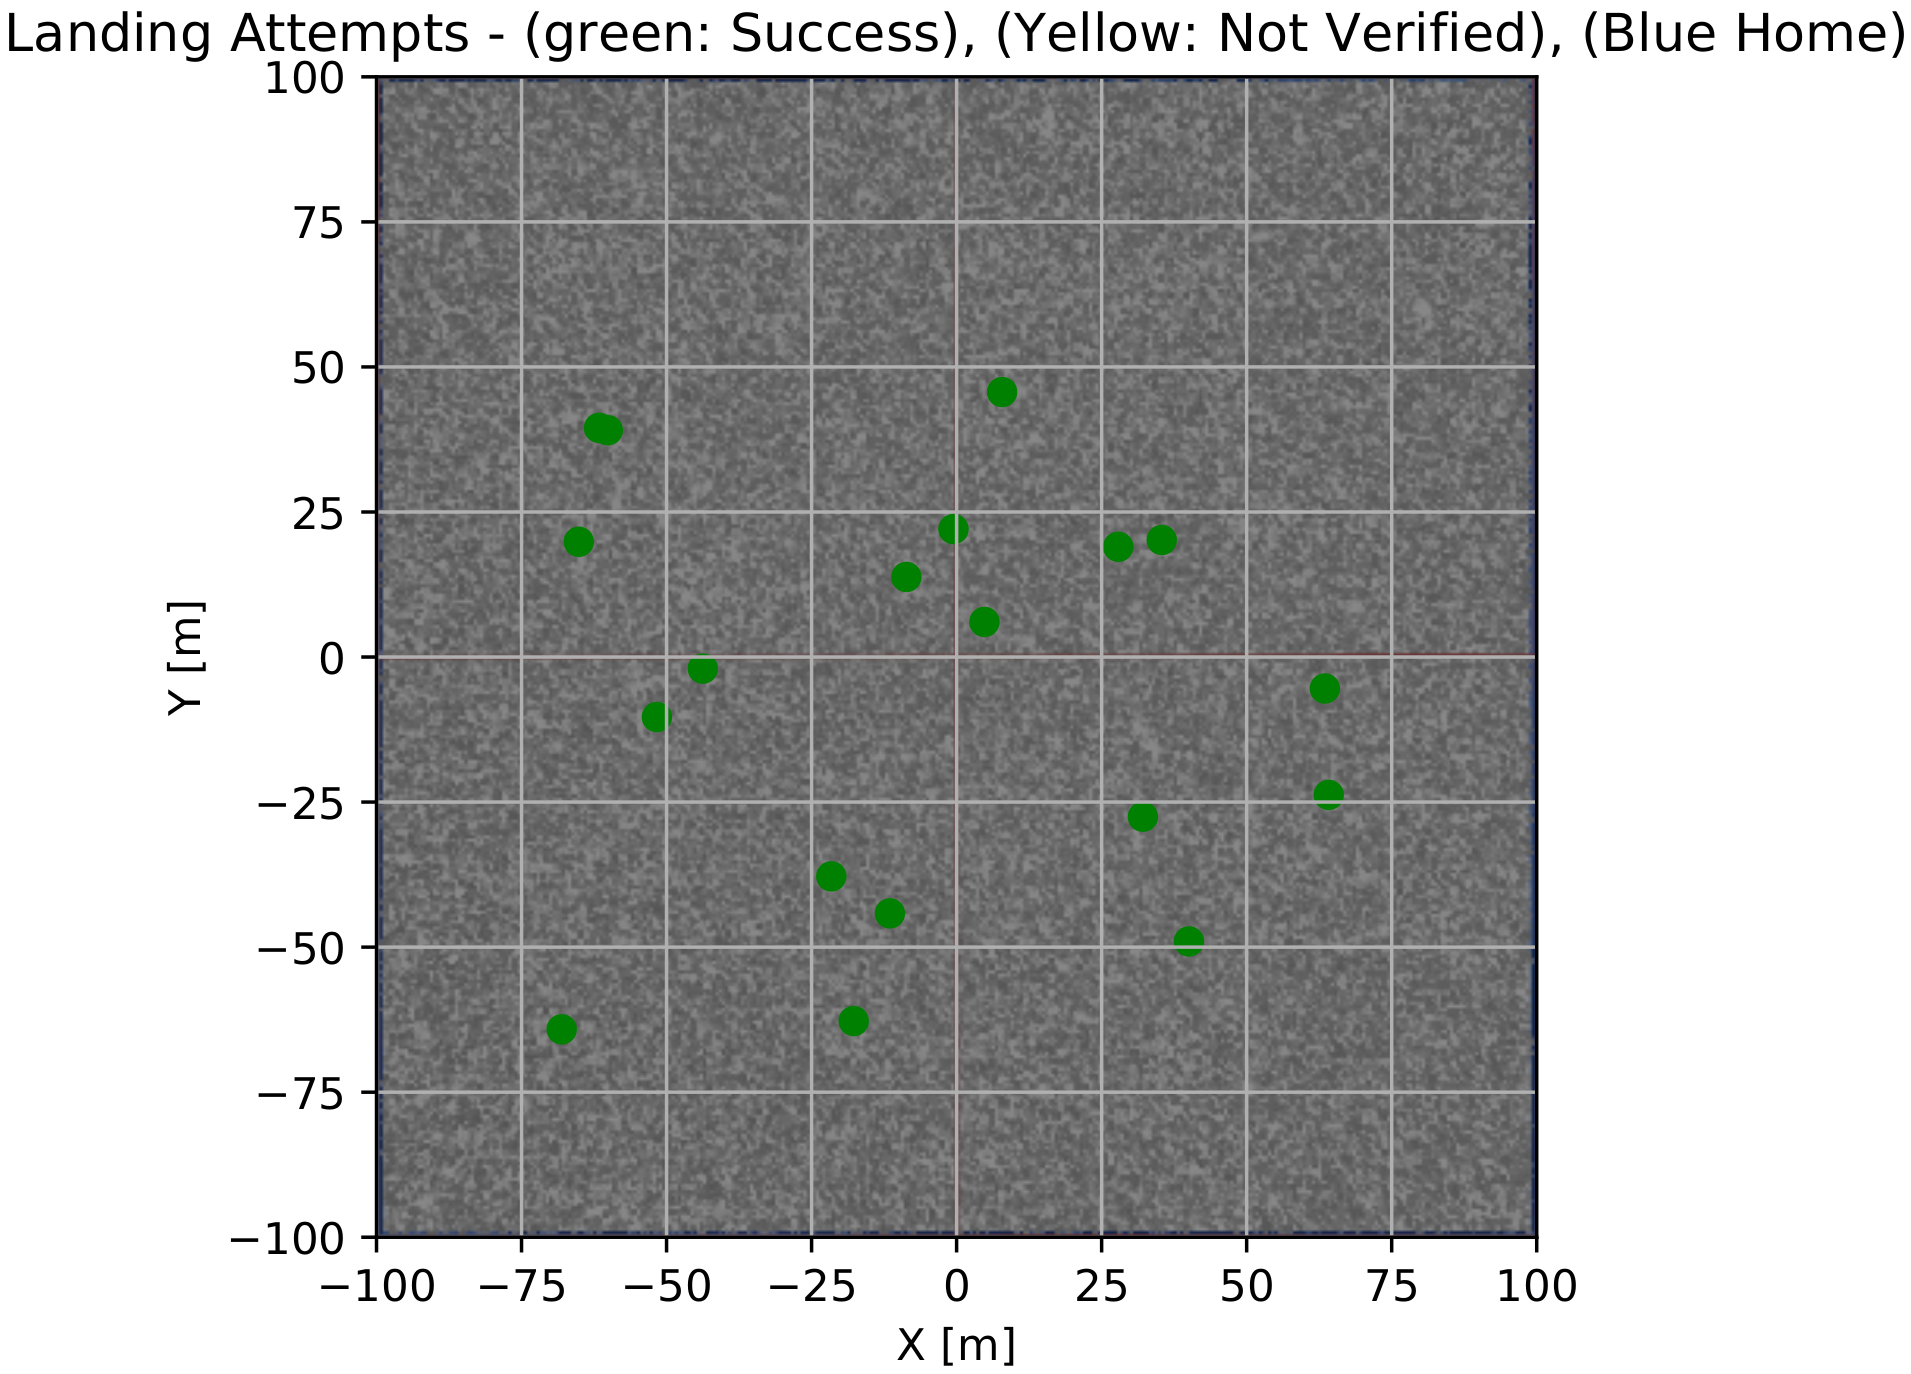
\includegraphics[scale=0.5]{images/evaluation/landing_rough_covered.png}
        \caption{Landing attempt locations for the rough map with platform covered by the mission}
        \label{fig:land_rough_covered}
        \end{figure}

        As both the spawn platform and the landing platforms were spawned randomly, evaluating the visual outcome is redundant. For the sake of completion, however, it is still displayed in \cref{fig:land_rough_covered}.

        \subsubsection{Numerical Discussion}
        One timeout occurred, and one verification failed. The residual flights all succeeded on the first landing site detected.

        % This proves that LSD does in fact not perceive convincing landing sites where there should be none. Additionally, as the drone never went home, this proves that LSD also detects landing sites where there should be safe landing zones.
        
        All landing site candidates except one were verified. This convincing result is not surprising as the inserted landing sites are of very high quality, and are therefore unlikely to trigger a verification failure. The verification rate is not perfect, however, as the landing sites were only thin disks, as shown in \cref{fig:rough_map_platform}. 

        To determine the pipeline's ability to choose the best available landing area, the final landing locations were compared to the platforms spawned. This was the result:

        \begin{table}[h]
            \begin{center}
             \caption{Final Landing Platform Choice}\vspace{1ex}
             \label{tab:final_landing_platform}
             \begin{tabular}{|c|c|c|c|}
             \hline
             \# Landings & \# On Earth (spawn) & \# Moon (1st pf)  & \# Mars (2nd pf)\\ \hline \hline
             99 & 4 & 2 & 93 \\
             \hline
            \end{tabular}
        \end{center}
        \caption{Landing locations chosen by this experiment - The Earth platform denotes the small spawn location of the drone. The Moon corresponds to the platform covered by the first mission waypoint, and the Mars platform is where the missions ended.}
        \end{table}

        This result shows, as desired, that the last platform, which is the one closest to the drone at the time of the last waypoint, was chosen most of the time. 
        
        When the Earth platform, which is the takeoff location, was close enough to the last waypoint, it was sometimes chosen because the landing sites discovered on it during takeoff were detected closer above ground than the ones at course altitude.

        The same happened when the first platform could be seen during ascent and was relatively close to the last waypoint.

\clearpage%HERE
\subsection{Rough Map - Random Waypoints}\label{subsec:rough_map_rw}

    \begin{figure}[h]
        \centering
        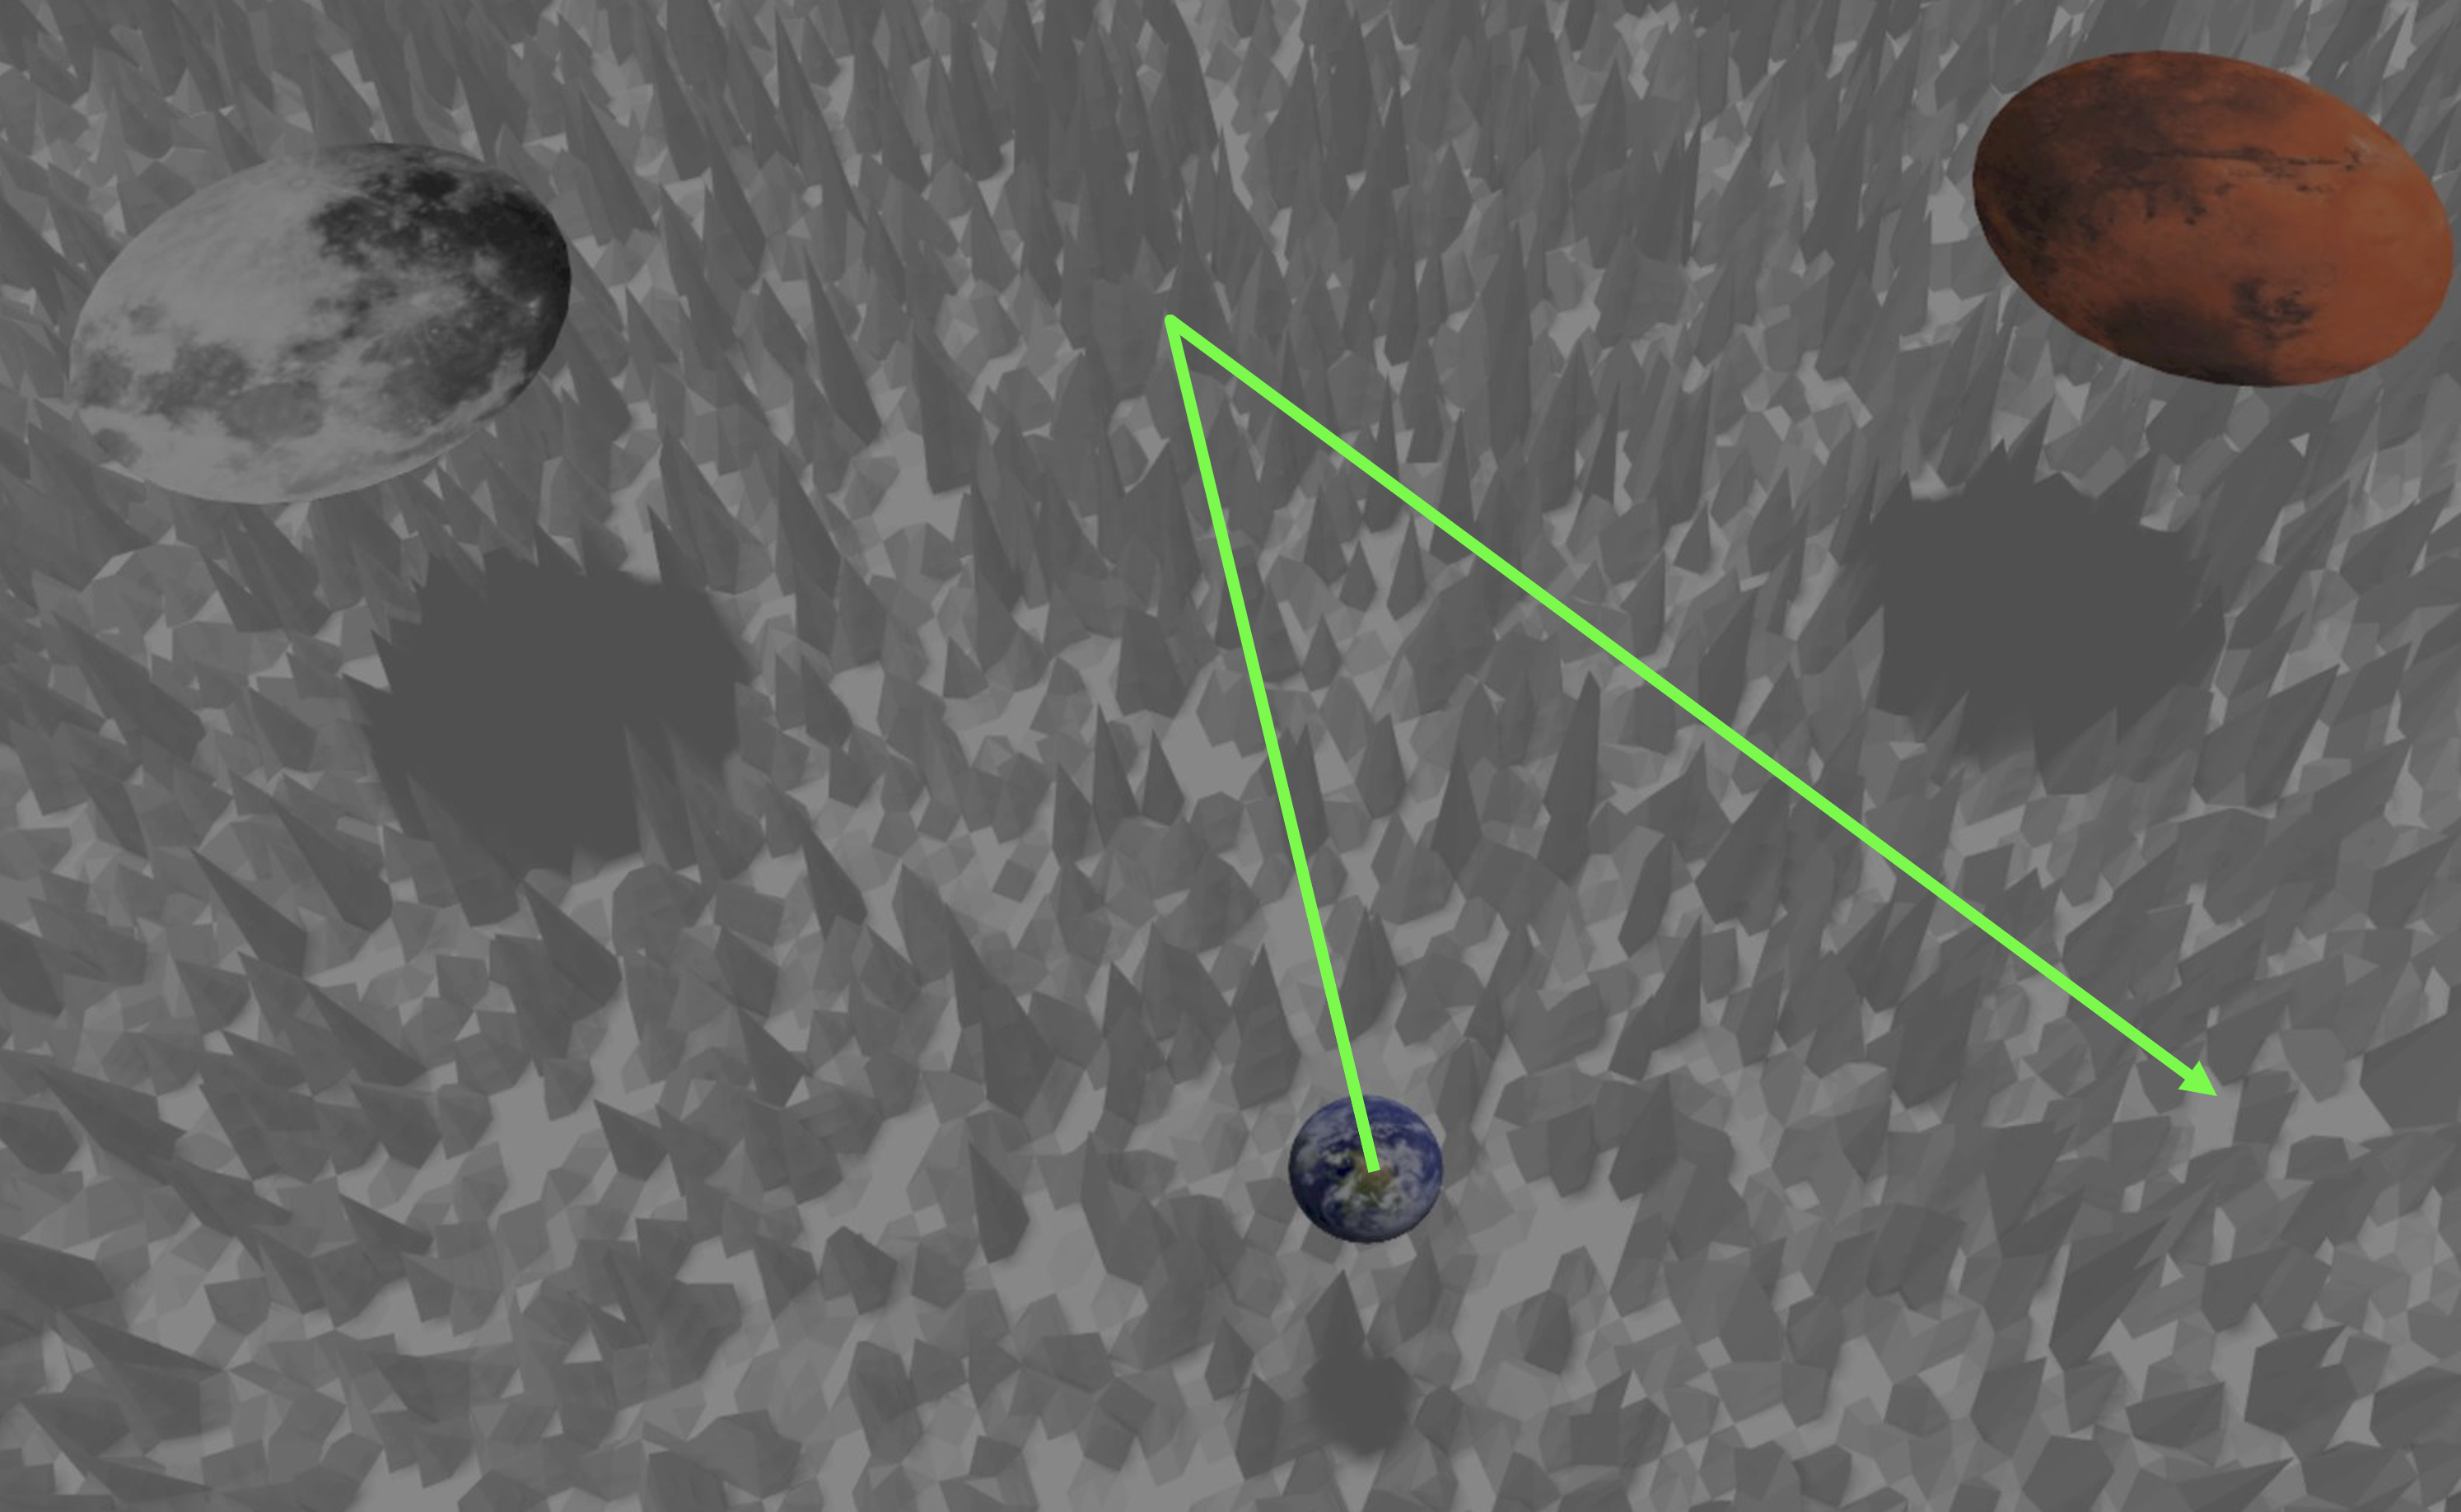
\includegraphics[scale=0.24]{images/evaluation/rough_complete_rand.png}
        \caption{Test flights on rough map with waypoints covering the landing sites}
        \label{fig:rough_compl_rand}
    \end{figure}

    In this test, changing the setup a bit, the drone flew a completely randomized two-waypoint pattern without the guarantee of flying over a safe landing site. This test set analyzed the pipeline's capabilities to deal with the case when no landing sites are detected initially.

    First, in this experiment of 100 flights, when the drone did not detect any landing sites, it flew only minimal landing site search patterns within a 1 m radius. This should serve as a baseline to see how many sites are approximately found without significant additional search actions.

    The numerical result thereof is displayed below:

    \begin{table}[h]
        \begin{center}
         \caption{Results - Rough map with platform coverage}\vspace{1ex}
         \label{tab:result_rough_rand}
         \begin{tabular}{|c|c|c|c|c|}
         \hline
         \# Flights & \# Successes & \# Con. Losses & \# Crashes & \# Home Landing\\ \hline \hline
         100 & 98 & 2 & 0 & 54 \\
         \hline
         \end{tabular}
        \end{center}
    \end{table}

    \begin{table}[h]
        \begin{center}
         \caption{Landing attempts rough map without platform covering mission}\vspace{1ex}
         \label{tab:land_nums_rough_rand}
         \begin{tabular}{|c|c|c|c|}
         \hline
         \# LS landings & \# Landing on first attempt & \# 2 attempts & \# 3 attempts\\ \hline \hline
         44 & 43 & 1 & 0 \\
         \hline
         \end{tabular}
        \end{center}
    \end{table}

    \begin{figure}[h]
    \centering
    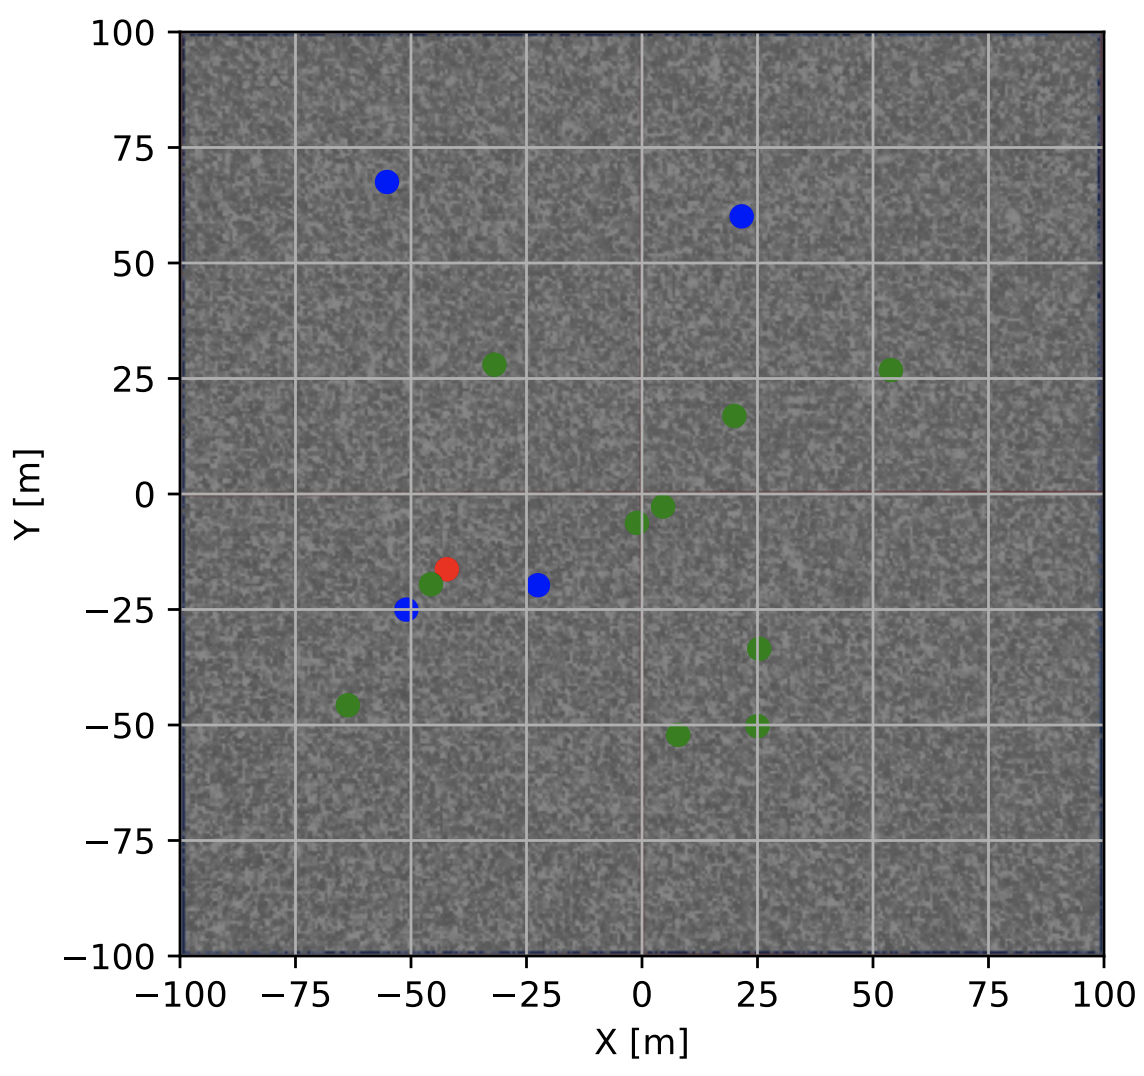
\includegraphics[scale=0.5]{images/evaluation/landing_rough_rand.png}
    \caption{Landing attempt locations for the rough map with completely random missions}
    \label{fig:land_rough_rand}
    \end{figure}

    \subsubsection{Numerical Discussion}

    Looking at \cref{tab:result_rough_rand}, what stands out are the 54 times the drone went to the home position. This is the desired behavior when no landing site is found, and it is therefore to be considered a success. It is also rather expected as the minimal search pattern radius likely prevents the drone from finding additional landing sites. Like for the case when the platforms were covered by the mission waypoints, the landing sites were almost always verified as they were of high quality by design. 
    

\subsection{Rough Map - Random WPs with Larger Search Radius}

    When flying the same experiment setup as introduced in \cref{subsec:rough_map_rw} but with a larger search pattern radius, we arrive at the following outcome:

    \begin{table}[h]
        \begin{center}
         \caption{Results - Rough map with platform coverage}\vspace{1ex}
         \label{tab:result_rough_rand_lr}
         \begin{tabular}{|c|c|c|c|c|}
         \hline
         \# Flights & \# Successes & \# Con. Losses & \# Crashes & \# Home Landing\\ \hline \hline
         100 & 98 & 2 & 0 & 34 \\
         \hline
         \end{tabular}
        \end{center}
    \end{table}

    \begin{table}[h]
        \begin{center}
         \caption{Landing attempts rough map without platform covering mission}\vspace{1ex}
         \label{tab:land_nums_rough_rand_lr}
         \begin{tabular}{|c|c|c|c|}
         \hline
         \# LS Landings & \# Landing on first attempt & \# 2 attempts & \# 3 attempts\\ \hline \hline
         66 & 60 & 6 & 0 \\
         \hline
         \end{tabular}
        \end{center}
    \end{table}

    \begin{figure}[h]
    \centering
    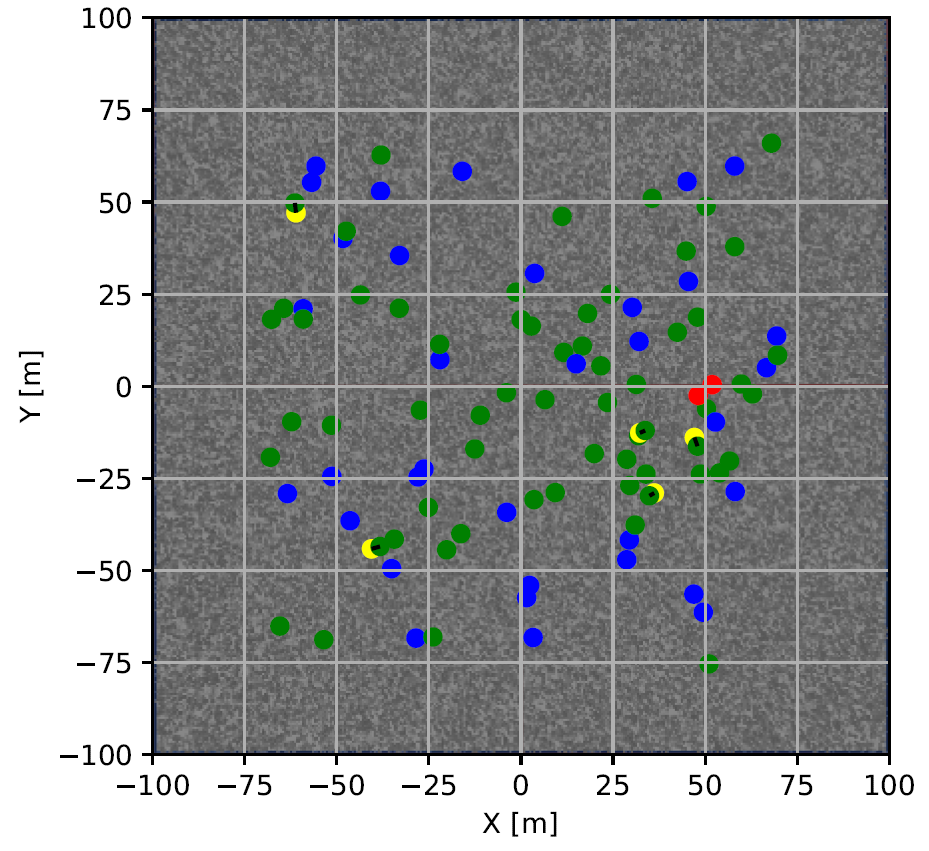
\includegraphics[scale=0.5]{images/evaluation/landing_rough_rand_lr.png}
    \caption{Landing attempt locations for the rough map with completely random missions and an increased landing site search action radius}
    \label{fig:land_rough_rand_radius}
    \end{figure}

    \subsubsection{Numerical Discussion}

    Compared to the same randomized run on the hostile terrain shown in \cref{subsec:rough_map_rw}, the drone went home only 34 times as opposed to the previous 54. This shows the impact of the additional search patterns flown when no platforms are seen during the mission. 

    6 times a second landing site had to be chosen. These were all picked on the same platform the initial landing was attempted. 
    
\clearpage%HERE

\subsection{Arroyo - Randomized Takeoff and Mission with SFM}\label{subsec:SFM_complete_rand}

    As mentioned in \cref{subsec:sfm_insufficiencies}, SFM's implementation at the time of this work was not well suited for high-altitude flights. For the sake of completeness, however, the pipeline was flown with SFM and analyzed in the following. 

    The setup was the same as for \cref{subsec:compl_rand} with randomized spawn and mission locations. However, this time, SFM was used to generate depth.

    \begin{table}[h]
        \begin{center}
            \caption{Results - SFM with random spawn and way points}\vspace{1ex}
            \label{tab:result_SFM}
            \begin{tabular}{|c|c|c|c|c|}
            \hline
            \# Flights & \# Successes & \# Con. Losses & \# Timeouts & \# Home Landing\\ \hline \hline
            100 & 77 & 18 & 5 & 0 \\ 
            \hline
            \end{tabular}
        \end{center}
    \end{table}

    \begin{table}[h]
        \begin{center}
            \caption{Landing attempts of successful flights when flown with SFM}\vspace{1ex}
            \label{tab:land_nums_SFM}
            \begin{tabular}{|c|c|c|c|}
            \hline
            \# Flights & \# 1st attempt & \# 2 attempts & \# 3 attempts\\ \hline \hline
            77 & 45 & 30 & 2   \\
            \hline
            \end{tabular}
        \end{center}
    \end{table}

    \begin{figure}[h]
    \centering
    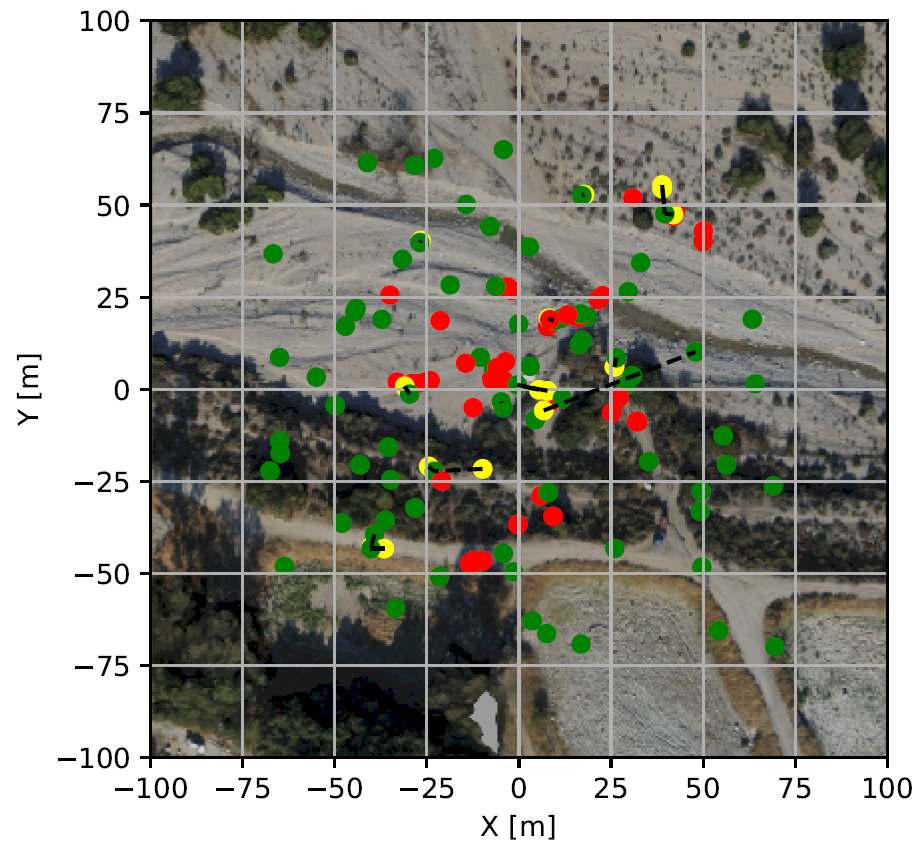
\includegraphics[scale=0.45]{images/evaluation/landing_SFM.png}
    \caption{Landing attempt locations when flying a mission with randomized drone spawns and randomized waypoints with SFM}
    \label{fig:land_SFM} 
    \end{figure}


    \subsubsection{Numerical Discussion}
    Compared to the other tests, in this setting, many connection losses occurred. 
    
    Additionally, the nominal procedure timed out five times, meaning that numerous landing site verifications were necessary, which ultimately prevented the flight from completing within the 10 minutes before the next iteration was started. 

    This occurred because of the following reasons:

    \begin{itemize}
        \item The landing site proposals supplied by SFM are of less quality than the ground truth leading to a higher probability of necessitating the selection of another landing site. 
        \item Secondly, overruling SFM measurements using stereo inputs takes substantial time. In practice the 15 s verification duration was not always sufficient to yield good estimates of the surrounding. Because of this, further landing sites of lower quality were selected, which were detected on SFM data from 100 m altitude. This led to further failures. Secondly, these landing sites were also more often farther away, which made the procedure slower.
    \end{itemize}

    This definitely has to be accounted for. As mentioned in \cref{subsubsec:setup:aggregation}, a potential remedy for excessive convergence could be time inflation of the OMG cells of the elevation map.
    
    \subsubsection{Visual Discussion}
    The first thing to note is the high number of red points. This is both because of the numerous connection losses and because of the landing attempts, which took too long and, therefore, didn't lead to a landing. The landing sites are, in general, of lesser quality than for the GT cases. Lastly, as can be seen in a successful run, subsequent landing sites were not always close by. As previously mentioned, this occurred when the stereo measurements did not overwrite the SFM information in time, so other, far-away SFM landing sites were selected.

\section{Theoretical Edge Cases}
\cref{sec:test_flights} shows that the implemented landing procedure performs well on terrain that is roughly comparable to that on Mars. These tests represent rather ordinary cases, though. In the following, a number of theoretical edge cases are introduced, and their handling by this work's pipeline is discussed.

\subsection{Arrival on Mars}
One concept for the rotorcraft's arrival on Mars is its takeoff during the descent of the main payload. In the Mars Sample Return mission, which has since been aborted, for instance, this payload would have been the landing platform to which the Mars samples would be returned. From that lander, the rotorcraft would take off mid-descent and land on its own.

Playing this scenario through, a small mission or pattern needs to be flown in order to move laterally and thus detect landing sites. Additionally, as the platform from which we took off is descending with neck-breaking velocity, we need to consider a different location for the choice of our home position. This can be done prior to the flight using a mixture of HiRISE images and information provided by Opportunity and Ingenuity. The ladder two options also ensure a sufficient image resolution to determine a home position safely.

If a landing site is successfully detected during this mission, the landing procedure is initiated as usual. If no candidates for suitable landing areas are found, however, further landing site search patterns at random locations are flown. If the landing site buffer remains empty, the aforementioned synthetic home position is navigated to and landed at.

\subsection{Flying on Large Scale Inclined Terrain}
The tests performed all happened on generally even terrain with rough and inclined areas spread throughout. What happens, however, when we want to fly the drone over large-scale inclined terrain? An example of this could be flying out of the Jezero crater which is where the Opportunity rover was deployed.

In this case, the necessary precautions must be taken during the mission planning stage. Assuming a mission was created at a cruise altitude high enough to allow lateral traversal to the farthest mission waypoint without danger of collision, the landing behavior would be the same. 

Two possible break points exist, however:

\begin{itemize}
    \item Lack of number and quality of landing sites

    Fewer landing sites are detected on inclined terrain. Secondly, a pipeline blind spot is unstable landing sites like larger rocks. Though the probability of landing on such a rock and thus making it fall over is very small, they exist, even more so on inclined terrain.

    \item Collision danger when flying LS search patterns

    The mission waypoints are set deterministically. Therefore, the terrain can be accounted for during their creation. 
    
    This is not the case for the random flight patterns executed when no landing sites are available. The center point of a rectangular search pattern is set randomly at a fixed distance from the location where the action was invoked. If, during the mission, a landing site was found at a very high altitude and turned out to be a false candidate, the LS search is initiated at that location. This case is schematically depicted in \cref{fig:search_pattern_collision}. Note how the landing site was detected at a significant distance from the last mission waypoint. 

    \begin{figure}[h]
        \centering
        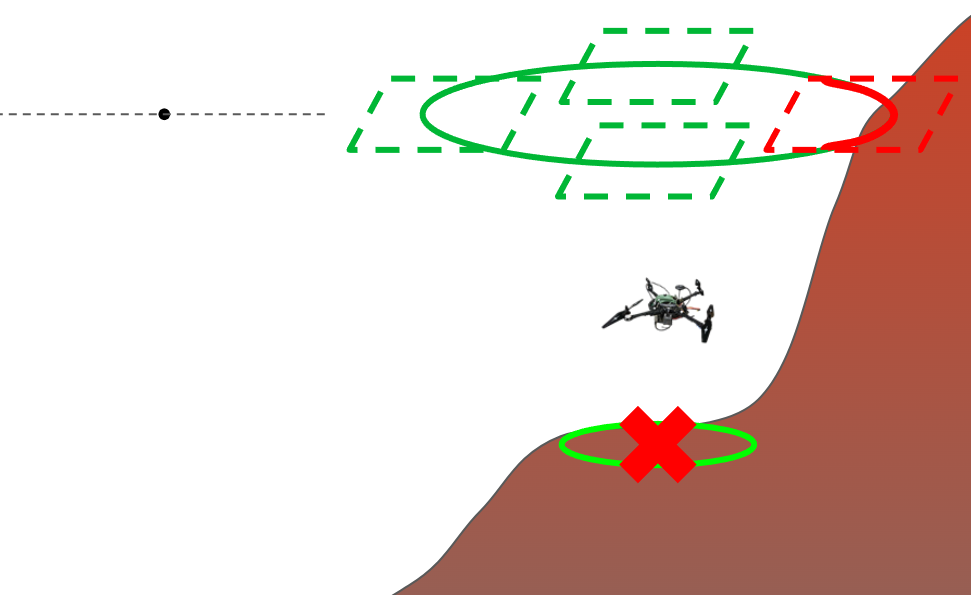
\includegraphics[scale=0.35]{images/evaluation/search_pattern_collision.png}
        \caption{Break case of landing site search pattern. The black dot indicates the last mission waypoint at cruise altitude. The bright green circle with the red cross shows an invalid landing site, and the circle above the drone shows the possible center points of search patterns.}
        \label{fig:search_pattern_collision}
    \end{figure}
\end{itemize}

One more break case for the presented pipeline is overhanging terrain. In that case, the ascent to a clearing altitude does not constitute a safe approach.

It must be noted, however, that the exploration of terrain as advanced as overhanging ground and cave systems is not considered part of the LORNA endeavor.
